\documentclass[12pt,a4paper,oneside]{report}
\usepackage[T1]{fontenc}
\usepackage[utf8]{inputenc}
\usepackage{mathptmx}
\usepackage{amsmath,amssymb}
\usepackage[left=3cm,right=2.5cm,top=2.5cm,bottom=2.5cm]{geometry}
\usepackage{setspace}
\usepackage{graphicx}
\usepackage{longtable,array,booktabs}
\usepackage[table]{xcolor}
\usepackage{caption}
\usepackage{chngcntr}
\usepackage{fancyhdr}
\usepackage{titlesec}
\usepackage{enumitem}
\usepackage[hidelinks]{hyperref}
\usepackage[T1]{fontenc}

\graphicspath{{../assets/}}
\definecolor{headfill}{HTML}{D9E2F3}
\setstretch{1.25}
\setlength{\parindent}{0pt}
\setlength{\parskip}{6pt}
\sloppy
\emergencystretch=2em
\counterwithout{figure}{chapter}
\counterwithout{table}{chapter}
\captionsetup{font=bf,labelsep=colon,skip=6pt}
\captionsetup[table]{position=top}
\setlist{itemsep=2pt,topsep=2pt}
\newcommand{\code}[1]{{\small\ttfamily #1}}

\titleformat{\chapter}[hang]{\bfseries\fontsize{20}{24}\selectfont}{\thechapter}{0.7em}{}
\titlespacing*{\chapter}{0pt}{0pt}{18pt}
\titleformat{\section}{\bfseries\fontsize{15}{18}\selectfont}{\thesection}{0.6em}{}
\titlespacing*{\section}{0pt}{14pt}{6pt}
\titleformat{\subsection}{\bfseries\fontsize{13}{16}\selectfont}{\thesubsection}{0.6em}{}
\titlespacing*{\subsection}{0pt}{10pt}{4pt}

\pagestyle{fancy}
\fancyhf{}
\fancyhead[L]{\small\itshape Secure Audits: Digital Evidence and Investigation Support System}
\fancyfoot[C]{\thepage}
\renewcommand{\headrulewidth}{0.4pt}
\fancypagestyle{plain}{\fancyhf{}\fancyfoot[C]{\thepage}\renewcommand{\headrulewidth}{0pt}}

\newcommand{\collegehead}{%
  \begin{center}
    {\Large\bfseries ST JOSEPH ENGINEERING COLLEGE}\\[2pt]
    {\bfseries An Autonomous Institution}\\
    {\small (Affiliated to VTU Belagavi, Recognized by AICTE)}\\
    {\bfseries Vamanjoor, Mangaluru - 575028, Karnataka}\\[6pt]
    {\bfseries DEPT. OF COMPUTER SCIENCE AND ENGINEERING}\\[6pt]
    
\includegraphics[height=2.4cm]{sjeclogo.png}
  \end{center}}

\begin{document}

\thispagestyle{empty}
\begin{center}
{\large\bfseries Visvesvaraya Technological University, Belagavi -- 590018}\\[8pt]

\includegraphics[height=2.8cm]{vtu.png}\\[10pt]
{\bfseries PROJECT REPORT}\\
{\bfseries ON}\\[8pt]
{\fontsize{18}{22}\selectfont\bfseries SECURE AUDITS: DIGITAL EVIDENCE AND\\INVESTIGATION SUPPORT SYSTEM}\\[6pt]
{\small\itshape Submitted in partial fulfillment for the award of degree of}\\[8pt]
{\large\bfseries BACHELOR OF ENGINEERING}\\ {\bfseries in}\\ {\large\bfseries COMPUTER SCIENCE \& ENGINEERING}\\[10pt]
{\bfseries\itshape Submitted by}\\[4pt]
\begin{tabular}{lr}
\textbf{Alisha Anton Fernandis} & \textbf{4SO20CS017} \\
\textbf{Amisha Josna Dsouza} & \textbf{4SO20CS019} \\
\textbf{Ancilla Teresa Dsouza} & \textbf{4SO20CS026} \\
\textbf{Apeksha A Govekar} & \textbf{4SO20CS031}
\end{tabular}\\[10pt]
{\bfseries\itshape Under the Guidance of}\\[2pt]
{\bfseries Ms Shivangi M}\\
{\small Assistant Professor, Department of CSE}\\[8pt]

\includegraphics[height=2.6cm]{sjeclogo.png}\\[6pt]
{\bfseries DEPT. OF COMPUTER SCIENCE AND ENGINEERING}\\
{\large\bfseries ST JOSEPH ENGINEERING COLLEGE}\\
{\bfseries An Autonomous Institution}\\
{\small (Affiliated to VTU Belagavi, Recognized by AICTE)}\\
{\bfseries Vamanjoor, Mangaluru - 575028, Karnataka}\\[8pt]
{\bfseries 2026-27}
\end{center}
\clearpage
\pagenumbering{roman}
\setcounter{page}{1}

\collegehead
\begin{center}{\Large\bfseries CERTIFICATE}\end{center}
\vspace{4pt}
Certified that the project work entitled \textbf{``Secure Audits: Digital Evidence and Investigation Support System''} carried out by
\begin{center}
\begin{tabular}{ll}
\textbf{Alisha Anton Fernandis} & \textbf{4SO20CS017} \\
\textbf{Amisha Josna Dsouza} & \textbf{4SO20CS019} \\
\textbf{Ancilla Teresa Dsouza} & \textbf{4SO20CS026} \\
\textbf{Apeksha A Govekar} & \textbf{4SO20CS031}
\end{tabular}
\end{center}
the bonafide students of VII semester Computer Science \& Engineering in partial fulfillment for the award of Bachelor of Engineering in Computer Science and Engineering of the Visvesvaraya Technological University, Belagavi during the year 2026-27. It is certified that all corrections/suggestions indicated during Internal Assessment have been incorporated in the report. The project report has been approved as it satisfies the academic requirements in respect of project work prescribed for the said degree.

\vspace{1.2cm}
\begin{tabular}{p{4.6cm}p{4.6cm}p{4.6cm}}
\rule{4cm}{0.4pt} & \rule{4cm}{0.4pt} & \rule{4cm}{0.4pt}\\
\textbf{Ms Shivangi M} & \textbf{Dr Melwyn D'Souza} & \textbf{Dr Rio D'Souza}\\
Project Guide & HOD-CSE & Principal
\end{tabular}

\vspace{0.8cm}
\textbf{External Viva:}\\[4pt]
\begin{tabular}{p{7.5cm}p{6cm}}
Examiner's Name & Signature with Date\\[8pt]
1. \dotfill & \dotfill\\[8pt]
2. \dotfill & \dotfill
\end{tabular}
\clearpage

\collegehead
\begin{center}{\Large\bfseries DECLARATION}\end{center}
We hereby declare that the entire work embodied in this Project Report titled \textbf{``Secure Audits: Digital Evidence and Investigation Support System''} has been carried out by us at St Joseph Engineering College, Mangaluru under the supervision of \textbf{Ms Shivangi M}, for the award of \textbf{Bachelor of Engineering} in \textbf{Computer Science \& Engineering}. This report has not been submitted to this or any other University for the award of any other degree.

\vspace{6pt}
\begin{tabular}{p{6.5cm}p{4cm}p{4cm}}
\textbf{Name} & \textbf{USN} & \textbf{Signature}\\[4pt]
Alisha Anton Fernandis & 4SO20CS017 & \\[4pt]
Amisha Josna Dsouza & 4SO20CS019 & \\[4pt]
Ancilla Teresa Dsouza & 4SO20CS026 & \\[4pt]
Apeksha A Govekar & 4SO20CS031 &
\end{tabular}
\clearpage

\begin{center}{\Large\bfseries Acknowledgement}\end{center}
We dedicate this page to acknowledge and thank those responsible for the shaping of the project. Without their guidance and help, the experience while constructing the dissertation would not have been so smooth and efficient.

We sincerely thank our Project Guide, \textbf{Ms.\ Shivangi M}, Assistant Professor, Department of Computer Science and Engineering, for her guidance and valuable suggestions which helped us to complete this project. We also thank our Project Coordinator, Department of Computer Science and Engineering, for their consistent encouragement.

We owe a profound gratitude to \textbf{Dr.\ Melwyn D'Souza}, Head of the Department, Computer Science and Engineering, whose kind support and guidance helped us to complete this work successfully.

We are extremely thankful to our Principal, \textbf{Dr.\ Rio D'Souza}, Director, \textbf{Rev.\ Fr.\ Wilfred Prakash D'Souza}, and Assistant Director, \textbf{Rev.\ Fr.\ Kenneth Rayner Crasta}, for their support and encouragement.

We would like to thank all faculty and staff of the Department of Computer Science and Engineering who have always been with us, extending their support, valuable suggestions, guidance, and encouragement throughout the project.

We also extend our gratitude to our friends and family members for their continuous support.
\clearpage
\begin{center}{\Large\bfseries Abstract}\end{center}
Digital evidence such as First Information Reports (FIRs), scanned documents, photographs, video and audio recordings plays a central role in criminal investigations. Its value depends on two things: the evidence must be analysed efficiently, and it must be demonstrably unchanged since collection. Investigators, however, often work with several unconnected tools, with multilingual documents, and with records of access that are difficult to defend.

Secure Audits: Digital Evidence and Investigation Support System is a web-based platform that places case management, evidence handling and forensic analysis behind one authenticated workflow. A React and TypeScript front end communicates with a FastAPI gateway that enforces role-based access control, stores evidence through a provider-agnostic storage gateway (local disk or S3-compatible object storage such as Cloudflare R2) and records every significant action in an audit log. Each uploaded file is fingerprinted with SHA-256 and its digest is registered in the EvidenceRegistry smart contract on an Ethereum-compatible network before the database record is committed. Verification recomputes the digest from the stored bytes and compares it with the database and the on-chain value, so that file tampering, missing files, unregistered evidence and database manipulation are reported as distinct outcomes.

Analysis modules are attached to the same evidence record: hybrid PaddleOCR and Tesseract text extraction for English, Hindi, Kannada, Telugu, Tamil and Malayalam documents with optional translation; YOLOv8-based object detection; Bharatiya Nyaya Sanhita (BNS) section decision support using sentence embeddings and statutory element matching; forensic audio analysis combining electric network frequency (ENF) tracking, splice and silence detection, WhisperX transcription and speaker diarization; and video-based 3D scene reconstruction using COLMAP and Open3D. A Person-Object-Location-Event (POLE) graph, investigator notes and a blockchain dashboard support the investigation workflow.

In the evaluation reported in this document, all 17 controlled integrity checks produced the expected outcome, hybrid OCR reduced the mean character error rate from 4.45\% to 1.18\%, the deployed BNS scorer recovered 91.5\% of manually assigned sections across 30 multi-offence FIRs, and video reconstruction achieved an observation-weighted reprojection error of 0.876 pixels.
\clearpage
\tableofcontents
\clearpage
\listoffigures
\clearpage
\listoftables
\clearpage
\pagenumbering{arabic}
\setcounter{page}{1}
\chapter{Introduction}
\section{Background}
The digitalisation of investigative and law-enforcement processes has increased reliance on electronic systems for managing criminal cases and evidence. Traditional case handling involves manual documentation, fragmented storage and limited traceability, which leads to inefficiency, inconsistent records and difficulty in demonstrating that evidence has remained intact. Modern investigations routinely involve images, scanned documents, audio and video, and tampering, unauthorised access or data loss can affect both the investigation and later legal proceedings. Transparent audit trails and chain-of-custody records are therefore essential.

In India, investigators also deal with documents written in several scripts, and with the Bharatiya Nyaya Sanhita (BNS), 2023, which replaced the Indian Penal Code and requires FIR narratives to be mapped to the new section numbering. These factors call for systems that combine secure evidence handling with multilingual document processing and legal decision support.

\textbf{Secure Audits: Digital Evidence and Investigation Support System} (referred to in this report as Secure Audit) is a multi-service platform that combines structured case management, secure evidence storage, cryptographic integrity verification, blockchain anchoring, audit logging and AI-assisted forensic analysis. It is built from a React front end, a FastAPI core gateway, four analysis microservices and an Ethereum smart contract, all coordinated around a single case and evidence record.

\section{Problem Statement}
Electronic records such as FIRs, images, videos and audio recordings can be altered, duplicated or accessed without authorisation, which weakens their reliability and evidentiary value. Many systems concentrate on storing evidence and do not provide an independent means of confirming that a file is unchanged after submission. The absence of a transparent chain of custody makes it difficult to establish who accessed evidence and what was done with it. Manual examination of large volumes of multimedia evidence is slow and prone to oversight, and the analysis tools used are usually separate from the system that records the evidence, so analysis results cannot be tied to a verified copy of the file.

Secure Audit addresses these problems by (i) fingerprinting every file on ingestion and anchoring the fingerprint on a blockchain, (ii) verifying stored evidence against both the database and the blockchain, (iii) recording custody events and audit entries for important actions, and (iv) attaching multilingual OCR, object detection, BNS decision support, audio forensics and 3D reconstruction to the same evidence record.

\section{Objectives}
\begin{enumerate}
  \item To develop a secure digital evidence management system with SHA-256 fingerprinting, tamper detection, chain-of-custody records and audit logging.
  \item To anchor evidence digests in an Ethereum smart contract and verify stored evidence against the file, the database record and the blockchain.
  \item To enforce authenticated, role-based access to cases, evidence and analysis functions.
  \item To provide AI-assisted analysis of digital evidence using multilingual OCR, object detection, forensic audio analysis and video-based 3D reconstruction.
  \item To assist investigators with BNS section identification, case relationship (POLE) visualisation and investigator notes within one platform.
\end{enumerate}

\section{Scope}
The system provides a centralised platform for creating cases, recording FIR details and uploading documents, images, audio and video as evidence. It covers hashing, storage, duplicate detection, blockchain registration, verification, custody records and audit logs; multilingual OCR and optional translation of scanned documents; YOLOv8 detection on image and video evidence; BNS decision support from FIR text; forensic audio analysis; video-based 3D reconstruction; and administrative functions such as user management and blockchain monitoring.

The platform is a decision-support and evidence-management tool. It does not make judicial decisions, perform real-time surveillance or connect to external law-enforcement databases. Analysis outputs are presented to investigators for review.

\section{Organisation of the Report}
Chapter 2 reviews related work. Chapter 3 specifies the requirements. Chapter 4 presents the system design, including architecture, data flow, database design, evidence storage, security and integrity mechanisms. Chapter 5 describes the implementation of each module and Chapter 6 explains the algorithms and technical methods used. Chapter 7 describes testing and validation, Chapter 8 presents results and discussion, Chapter 9 summarises applications, advantages and limitations, and Chapter 10 concludes the report.

\chapter{Literature Survey}
\section{Introduction}
Research relevant to Secure Audit spans digital evidence management, blockchain-based chain of custody, object detection, multilingual OCR, forensic audio analysis, 3D crime-scene reconstruction, legal text classification and knowledge-based investigation. This chapter reviews twelve representative works and identifies the gap that the proposed system addresses.

\section{Bonomi et al.: B-CoC, a Blockchain-Based Chain of Custody [1]}
Bonomi et al. proposed B-CoC, a blockchain-based approach for managing the chain of custody of digital evidence. Evidence-related operations are recorded on a distributed ledger, giving a tamper-evident history of handling. The work shows how distributed ledgers improve traceability and accountability, but it requires careful integration of ledger records with conventional forensic workflows. It motivates the evidence registration and verification mechanism in Secure Audit.

\section{Li et al.: LeChain, Lawful Evidence Management [2]}
LeChain applies blockchain technology to lawful evidence management, recording evidence information in a tamper-resistant manner. The study demonstrates the potential of blockchain for reliable evidence records; its practical integration with application-level storage and investigation workflows remains an implementation concern. Secure Audit adopts the same principle by registering SHA-256 evidence hashes on a blockchain and using the registered values in later verification.

\section{Sazaly et al.: 3D Indoor Crime Scene Reconstruction [3]}
Sazaly et al. combined micro-UAV imagery, processed with Structure from Motion, and terrestrial laser scanning to reconstruct indoor crime scenes, obtaining better accuracy than either source alone. Limitations include distortion on reflective surfaces, manual alignment and the absence of a chain-of-custody mechanism. This supports the photogrammetry module of Secure Audit.

\section{Balbudhe et al.: Crime Scene Reconstruction, a Scoping Review [4]}
The review covers laser scanning, photogrammetry, virtual reality and mixed reality for crime-scene reconstruction. It reports that laser scanning and photogrammetry are reliable and that immersive technologies can improve understanding, but it notes the lack of standard procedures, privacy concerns and computational cost.

\section{Mathias et al.: RAG-HGAT for BNS Section Classification [5]}
Mathias et al. proposed a retrieval-augmented hierarchical graph attention architecture for classifying BNS sections from complaint narratives, using LegalBERT embeddings, FAISS retrieval and graph attention. High performance was reported on a synthetic dataset; limitations include synthetic training data, incomplete BNS coverage and no OCR-based preprocessing.

\section{Kuok et al.: CrimeKGQA [6]}
CrimeKGQA combines a crime knowledge graph with retrieval-augmented generation to answer investigative queries. It shows the value of knowledge graphs for investigation, but depends on a proprietary language-model API and gives limited quantitative evaluation, raising cost, privacy and data-sovereignty concerns.

\section{Quyyum and Abdullah: Weapon Detection in Surveillance Video [7]}
An improved YOLOv3 approach with custom anchors, additional blurry CCTV images and an extra prediction layer improved mean average precision for weapon detection. It covers few weapon categories and is not integrated with evidence management.

\section{Ngharamike et al.: ENF-Based Multimedia Forensics [8]}
This survey describes extracting the electric network frequency from audio and video for time verification, tamper detection and location authentication. ENF analysis is difficult when the signal is weak or noisy and generally needs long recordings.

\section{Pedapudi and Vadlamani: Forensics for Audio and Video Files [9]}
The methodology uses MediaInfo and Sonic Visualiser for frame extraction, histogram comparison and hash verification. It depends on manual analysis, has no automated chain of custody and uses MD5 and SHA-1, which give weaker integrity protection than SHA-256.

\section{Al Sayem et al.: Tesseract for Information Extraction [10]}
The study evaluated Tesseract on business-card images and showed that OCR accuracy depends on image quality, colour and preprocessing. The dataset was small and does not represent degraded, multilingual investigative documents, which motivates a robust hybrid OCR pipeline.

\section{Dhanushkumar et al.: NLP and Generative AI in Law for BNS [11]}
The survey discusses retrieval-augmented generation, OCR and automated legal assistance for the BNS. It stresses retrieval for reliability but notes the lack of standard BNS benchmarks and limited regional-language support.

\section{Werukanjana and Permpool: Object Detection in Crime Scene Investigation [12]}
YOLOv8 transfer learning achieved high precision and recall for firearm-related objects in crime-scene images, using a relatively small dataset and without integration with evidence management or chain of custody.

\section{Comparison of Existing Methods}
Table 1 compares the reviewed works by method, reported result and limitation.

{\footnotesize
\setlength{\tabcolsep}{3pt}
\renewcommand{\arraystretch}{1.15}
\begin{longtable}{|>{\raggedright\arraybackslash}p{1.33cm}|>{\raggedright\arraybackslash}p{2.84cm}|>{\raggedright\arraybackslash}p{3.79cm}|>{\raggedright\arraybackslash}p{3.03cm}|>{\raggedright\arraybackslash}p{3.22cm}|}
\caption{Comparative analysis of existing work}\\
\hline
\rowcolor{headfill}\textbf{Ref.} & \textbf{Work} & \textbf{Methodology} & \textbf{Reported result} & \textbf{Limitation} \\ \hline
\endfirsthead
\hline
\rowcolor{headfill}\textbf{Ref.} & \textbf{Work} & \textbf{Methodology} & \textbf{Reported result} & \textbf{Limitation} \\ \hline
\endhead
\hline \endfoot
[1],[2] & Blockchain chain of custody & Ledger records of evidence operations & Tamper-evident history & Integration with workflows \\ \hline
[3] & 3D crime-scene reconstruction & UAV photogrammetry + laser scan fusion, SfM & RMSE 0.217 cm & Manual alignment; no audit integration \\ \hline
[4] & Reconstruction review & Photogrammetry, laser scanning, VR/MR & VR improves understanding by 25--30\% & Cost; no standardisation \\ \hline
[5] & BNS classification & RAG + LegalBERT + graph attention & 98.71\% micro F1 (synthetic data) & Synthetic data; limited BNS coverage \\ \hline
[6] & CrimeKGQA & Knowledge graph + RAG with LLM & Multi-hop query answering & No metrics; API dependency \\ \hline
[7] & Weapon detection & YOLOv3 anchor tuning, augmentation & 90.20\% mAP & Two classes; no forensic integration \\ \hline
[8] & ENF forensics & ENF via STFT and parametric methods & Up to 94.7\% accuracy & Needs long recordings \\ \hline
[9] & Audio/video forensics & Metadata, hashing, frame comparison & Effective tamper detection & Manual; weaker hashes \\ \hline
[10] & OCR with Tesseract & LSTM OCR with preprocessing & 96.87\% word accuracy & Poor on noisy images \\ \hline
[11] & AI in legal systems & RAG + OCR + LLM analysis & Up to 89\% accuracy & No deployment; limited languages \\ \hline
[12] & Object detection & YOLOv8 transfer learning & Precision 0.97 & Small dataset \\ \hline
\end{longtable}
}

\section{Research Gap and Proposed System}
The reviewed studies address individual problems well, but each is limited to one task, and none ties its analysis to a verifiable record of the evidence it consumed. Secure Audit integrates established techniques into one workflow: evidence is fingerprinted and anchored on a blockchain, stored through a controlled gateway, verified against independent references, and then analysed using OCR, object detection, BNS decision support, audio forensics and 3D reconstruction, with every significant action recorded in an audit log. The contribution of the project is this integration into a structured, traceable investigation environment rather than a new algorithm for any single task.

\chapter{Software Requirements Specification}
\section{Functional Requirements}
{\footnotesize
\setlength{\tabcolsep}{3pt}
\renewcommand{\arraystretch}{1.15}
\begin{longtable}{|>{\raggedright\arraybackslash}p{1.33cm}|>{\raggedright\arraybackslash}p{3.03cm}|>{\raggedright\arraybackslash}p{9.85cm}|}
\caption{Functional requirements}\\
\hline
\rowcolor{headfill}\textbf{ID} & \textbf{Function} & \textbf{Description} \\ \hline
\endfirsthead
\hline
\rowcolor{headfill}\textbf{ID} & \textbf{Function} & \textbf{Description} \\ \hline
\endhead
\hline \endfoot
FR-1 & Authentication & Two-step login: an OTP is e-mailed to the registered address and the officer submits the OTP and password to receive a signed JWT. Deactivated accounts are refused; new or reset accounts must change their password before use. \\ \hline
FR-2 & Role-based access & Roles Admin and Investigator determine the permissions to create cases, upload evidence, run AI analysis, view audit logs, manage users and see dashboard analytics. \\ \hline
FR-3 & Case and FIR management & Create cases with a generated case number, FIR description and language, complainant, victims, suspects, incident date, time and location; list, view and archive-flag cases; dashboard statistics. \\ \hline
FR-4 & Evidence upload & Upload files to a case with type and description; reject empty or oversized files (default 200 MB); compute SHA-256; detect duplicates within a case; flag duplicates across cases. \\ \hline
FR-5 & Evidence storage & Store files through a storage gateway (local disk or S3-compatible storage) under case-scoped keys with write-once semantics; authenticated download. \\ \hline
FR-6 & Blockchain registration & Register evidence ID, case ID, file name, SHA-256 and uploader in the EvidenceRegistry contract; persist the transaction receipt; do not save evidence if registration fails. \\ \hline
FR-7 & Integrity verification & Recompute SHA-256 from stored bytes and compare with the database and blockchain; report Verified, Tampered, Missing or Unregistered with a reason code; record the result. \\ \hline
FR-8 & Chain of custody & Maintain custody records (on-chain REGISTERED, VERIFIED, TRANSFERRED and database-only CREATED, VIEWED, DOWNLOADED, METADATA\_MODIFIED); allow custody transfer. \\ \hline
FR-9 & Audit logging & Record logins, uploads, verifications, tamper alerts, AI runs and administrative actions with user, case, hash, metadata and timestamp; provide filtered retrieval. \\ \hline
FR-10 & Multilingual OCR & Extract page-wise text from images and PDFs in English, Hindi, Kannada, Telugu, Tamil and Malayalam with confidence, detected languages and layout; optional translation. \\ \hline
FR-11 & Object detection & Run YOLOv8 detection on evidence images (and videos in the detection service) after an integrity check; return labels, confidences and bounding boxes. \\ \hline
FR-12 & BNS decision support & Return ranked BNS sections with confidence, severity, cognizability, bailability, punishment, trigger sentences and explanation; allow investigators to store accepted predictions. \\ \hline
FR-13 & Audio forensics & Analyse audio for ENF consistency, splicing and silence insertion, environment shifts, transcription, speaker segments and keywords; produce a tampering assessment. \\ \hline
FR-14 & 3D reconstruction & Create asynchronous reconstruction jobs from video evidence, report step-wise progress, and serve GLB and PLY outputs. \\ \hline
FR-15 & Investigation aids & POLE relationship graph for each case, personal notes, integrity alerts surfaced through audit status, and a blockchain dashboard with ledger, transaction and integrity-scan views. \\ \hline
FR-16 & User administration & Administrators create users, set roles and case-creation rights, activate or deactivate accounts and reset access. \\ \hline
\end{longtable}
}

\section{Non-Functional Requirements}
{\footnotesize
\setlength{\tabcolsep}{3pt}
\renewcommand{\arraystretch}{1.15}
\begin{longtable}{|>{\raggedright\arraybackslash}p{2.84cm}|>{\raggedright\arraybackslash}p{11.36cm}|}
\caption{Non-functional requirements}\\
\hline
\rowcolor{headfill}\textbf{Attribute} & \textbf{Requirement} \\ \hline
\endfirsthead
\hline
\rowcolor{headfill}\textbf{Attribute} & \textbf{Requirement} \\ \hline
\endhead
\hline \endfoot
Security & Bearer-JWT authentication on API calls; role and case-ownership checks; configurable CORS origins; secrets only in environment variables; filename sanitisation and path-traversal protection on storage keys; no public static exposure of evidence in the storage gateway. \\ \hline
Integrity & Evidence must be tamper-evident: any change to stored bytes, to the database hash or to registration metadata must be detectable and reported distinctly from missing or unreadable files. \\ \hline
Auditability & Important actions must produce audit records; verification outcomes caused by outages must not overwrite the true integrity state of evidence. \\ \hline
Reliability & Registration is transactional: the database commit happens only after the blockchain receipt is obtained, otherwise the upload is rolled back. Blockchain and storage outages return structured errors. \\ \hline
Modularity & Frontend, gateway, AI services, database, storage and blockchain are separate components that communicate through REST and Web3 JSON-RPC, so a service can be replaced or scaled independently. \\ \hline
Usability & Single-page interface with a dashboard, case workspace and dedicated pages for each analysis; clear error messages for failed operations. \\ \hline
Configurability & Storage backend, upload limit, OCR limits, blockchain timeouts and retries, translation providers and service URLs are controlled through environment variables. \\ \hline
Portability & Runs on Windows 10/11 or Linux; CPU execution is supported, GPU acceleration is used where available (COLMAP dense reconstruction requires CUDA). \\ \hline
\end{longtable}
}

\section{User Roles and Permissions}
Two roles are defined in the gateway's role-permission table. Administrators have unrestricted visibility, while investigators work with cases they own.

{\small
\setlength{\tabcolsep}{3pt}
\renewcommand{\arraystretch}{1.15}
\begin{longtable}{|>{\raggedright\arraybackslash}p{4.73cm}|>{\raggedright\arraybackslash}p{2.84cm}|>{\raggedright\arraybackslash}p{6.63cm}|}
\caption{Role-permission matrix}\\
\hline
\rowcolor{headfill}\textbf{Permission} & \textbf{Admin} & \textbf{Investigator} \\ \hline
\endfirsthead
\hline
\rowcolor{headfill}\textbf{Permission} & \textbf{Admin} & \textbf{Investigator} \\ \hline
\endhead
\hline \endfoot
create\_case & Yes & Yes (can be disabled per user by an administrator) \\ \hline
upload\_evidence & Yes & Yes \\ \hline
run\_ai\_analysis & Yes & Yes \\ \hline
generate\_storyboard & Yes & Yes \\ \hline
view\_cases & All cases & Owned cases only \\ \hline
view\_audit\_logs & All entries & Own entries only \\ \hline
dashboard\_analytics & All & Limited \\ \hline
manage\_users, system\_settings & Yes & No \\ \hline
\end{longtable}
}

\section{Hardware Requirements}
\begin{itemize}
  \item \textbf{Processor:} a multi-core CPU is sufficient for OCR, BNS scoring, audio analysis and detection; the evaluation in Chapter 8 used an Intel Core i5-1335U laptop (12 threads).
  \item \textbf{Memory:} 16 GB RAM is recommended when OCR, the BNS encoder and audio models are loaded together.
  \item \textbf{GPU:} an NVIDIA GPU with CUDA is required for COLMAP dense stereo (PatchMatch) and speeds up detection and transcription; other modules run on CPU.
  \item \textbf{Storage:} sufficient space for evidence files, reconstruction workspaces (frames, COLMAP databases, point clouds) and model weights.
\end{itemize}

\section{Software Requirements}
{\footnotesize
\setlength{\tabcolsep}{3pt}
\renewcommand{\arraystretch}{1.15}
\begin{longtable}{|>{\raggedright\arraybackslash}p{3.41cm}|>{\raggedright\arraybackslash}p{10.79cm}|}
\caption{Software environment}\\
\hline
\rowcolor{headfill}\textbf{Component} & \textbf{Technology and role} \\ \hline
\endfirsthead
\hline
\rowcolor{headfill}\textbf{Component} & \textbf{Technology and role} \\ \hline
\endhead
\hline \endfoot
Operating system & Windows 10/11 or Linux (Ubuntu 20.04 or later) \\ \hline
Frontend & React 18, TypeScript 5, Vite 5, React Router 6, Axios; Recharts (charts), @xyflow/react (POLE graph), Excalidraw (notes canvas), Three.js (3D viewer), Supabase JS client \\ \hline
Core backend & Python 3.10, FastAPI, Uvicorn, SQLAlchemy 2, psycopg2, PyJWT, bcrypt, Supabase client, Web3.py 7, boto3, requests \\ \hline
Database and identity & PostgreSQL (hosted through Supabase); Supabase Auth for user identities \\ \hline
Evidence storage & Local filesystem provider or S3-compatible provider (Cloudflare R2) via boto3 \\ \hline
Blockchain & Solidity 0.8.28 smart contract, Hardhat (compile and deploy), Ganache 7 local Ethereum node (chain ID 1337) \\ \hline
OCR and translation & PaddleOCR 3.x with PaddlePaddle 3.1 (PP-OCRv5 models), Tesseract 5 with script-specific models, pypdfium2/Poppler for PDF rendering, OpenCV, Pillow, deep-translator \\ \hline
Object detection & Ultralytics YOLOv8, OpenCV, NumPy \\ \hline
BNS service & sentence-transformers (all-MiniLM-L6-v2), PyTorch, NumPy; FAISS and PyTorch Geometric are included for the retrieval and graph-attention research components \\ \hline
Audio service & librosa, SciPy, soundfile, miniaudio, pydub/FFmpeg, WhisperX, pyannote.audio (optional diarization), SpeechRecognition \\ \hline
Photogrammetry & OpenCV, COLMAP (system binary), Open3D, SciPy, NumPy \\ \hline
\end{longtable}
}

\section{Environment Configuration}
Configuration is supplied through environment files that are excluded from version control. Only variable names and purposes are documented here; no values are recorded.

{\footnotesize
\setlength{\tabcolsep}{3pt}
\renewcommand{\arraystretch}{1.15}
\begin{longtable}{|>{\raggedright\arraybackslash}p{2.46cm}|>{\raggedright\arraybackslash}p{7.01cm}|>{\raggedright\arraybackslash}p{4.73cm}|}
\caption{Environment variables by service}\\
\hline
\rowcolor{headfill}\textbf{Service} & \textbf{Variables} & \textbf{Purpose} \\ \hline
\endfirsthead
\hline
\rowcolor{headfill}\textbf{Service} & \textbf{Variables} & \textbf{Purpose} \\ \hline
\endhead
\hline \endfoot
Core backend & SUPABASE\_URL, SUPABASE\_KEY, SUPABASE\_SERVICE\_ROLE\_KEY & Supabase project endpoint and keys \\ \hline
 & JWT\_SECRET & Signing key for session tokens \\ \hline
 & EMAIL\_USER, EMAIL\_PASSWORD, SMTP\_HOST, SMTP\_PORT, SMTP\_TIMEOUT\_SECONDS & SMTP delivery of OTP e-mails \\ \hline
 & DB\_HOST, DB\_PORT, DB\_NAME, DB\_USER, DB\_PASSWORD (or DATABASE\_URL) & PostgreSQL connection \\ \hline
 & STORAGE\_BACKEND, UPLOADS\_DIR, S3\_BUCKET\_NAME, S3\_ENDPOINT\_URL, S3\_REGION, S3\_ACCESS\_KEY\_ID, S3\_SECRET\_ACCESS\_KEY & Storage gateway provider selection and S3-compatible settings \\ \hline
 & ETHEREUM\_RPC\_URL, EVIDENCE\_REGISTRY\_ADDRESS, ETHEREUM\_SENDER\_ADDRESS, ETHEREUM\_PRIVATE\_KEY, BLOCKCHAIN\_* & Blockchain endpoint, contract, signer, timeouts, retries, confirmations and event polling \\ \hline
 & OCR\_*, POPPLER\_PATH, TESSERACT\_CMD, TRANSLATION\_* & OCR models, limits, preprocessing switches and translation providers \\ \hline
 & MAX\_UPLOAD\_MB, MAX\_HASH\_DOWNLOAD\_MB, ALLOWED\_ORIGINS, TRUST\_PROXY\_HEADERS & Upload and hashing limits, CORS origins, proxy handling \\ \hline
Detection service & MODEL\_PATH / BEST\_MODEL\_PATH, CONFIDENCE\_THRESHOLD, HOST, PORT & Model weights and default confidence \\ \hline
BNS service & MODEL\_DIR, LEGAL\_BERT\_NAME, SENT\_MODEL, FRONTEND\_ORIGIN, PORT & Model data and encoder names \\ \hline
Audio service & AUDIO\_HOST, PORT & Service binding \\ \hline
Photogrammetry & SUPABASE\_URL, SUPABASE\_SERVICE\_ROLE\_KEY, UPLOAD\_DIR, OUTPUT\_DIR, COLMAP\_BINARY, PORT & Job workspace, COLMAP location and database access \\ \hline
Frontend & VITE\_SUPABASE\_URL, VITE\_SUPABASE\_ANON\_KEY, VITE\_API\_BASE\_URL & Supabase public settings and API base URL \\ \hline
\end{longtable}
}

\section{Design Constraints}
\begin{itemize}
  \item \textbf{Legal scope:} the platform targets the Indian law-enforcement context and the BNS. The deployed scorer holds statutory profiles for 96 BNS section entries, and the research classifier was trained on 57 sections.
  \item \textbf{ENF analysis:} reliable ENF estimation needs a recording that contains mains hum; mobile recordings frequently lack it, in which case the result is reported as inconclusive.
  \item \textbf{Photogrammetry:} reconstruction needs overlapping, sharp views and may fail on reflective or featureless surfaces; dense stereo needs a CUDA GPU.
  \item \textbf{Blockchain network:} the provided deployment is a single-node Ganache development network; production use would require a permissioned or public network.
  \item \textbf{External services:} optional translation relies on third-party translation providers.
  \item \textbf{Detection model:} accuracy depends on the training classes and on image quality, illumination and occlusion.
\end{itemize}

\chapter{System Design}
This chapter presents the architecture of Secure Audit, the decomposition into modules, the data flow, the evidence workflows, the database and storage design, and the mechanisms for security, integrity and auditability.

\section{Architecture Design}
Secure Audit uses a layered, service-oriented architecture (Figure 1). The presentation layer is a React single-page application. All requests pass through a FastAPI core gateway that authenticates the caller, checks permissions and case ownership, and either handles the request directly or forwards it to an analysis microservice. Data is held in PostgreSQL and in an evidence store behind a storage gateway, while the blockchain layer provides an independent integrity reference.

\begin{figure}[htbp]
\centering
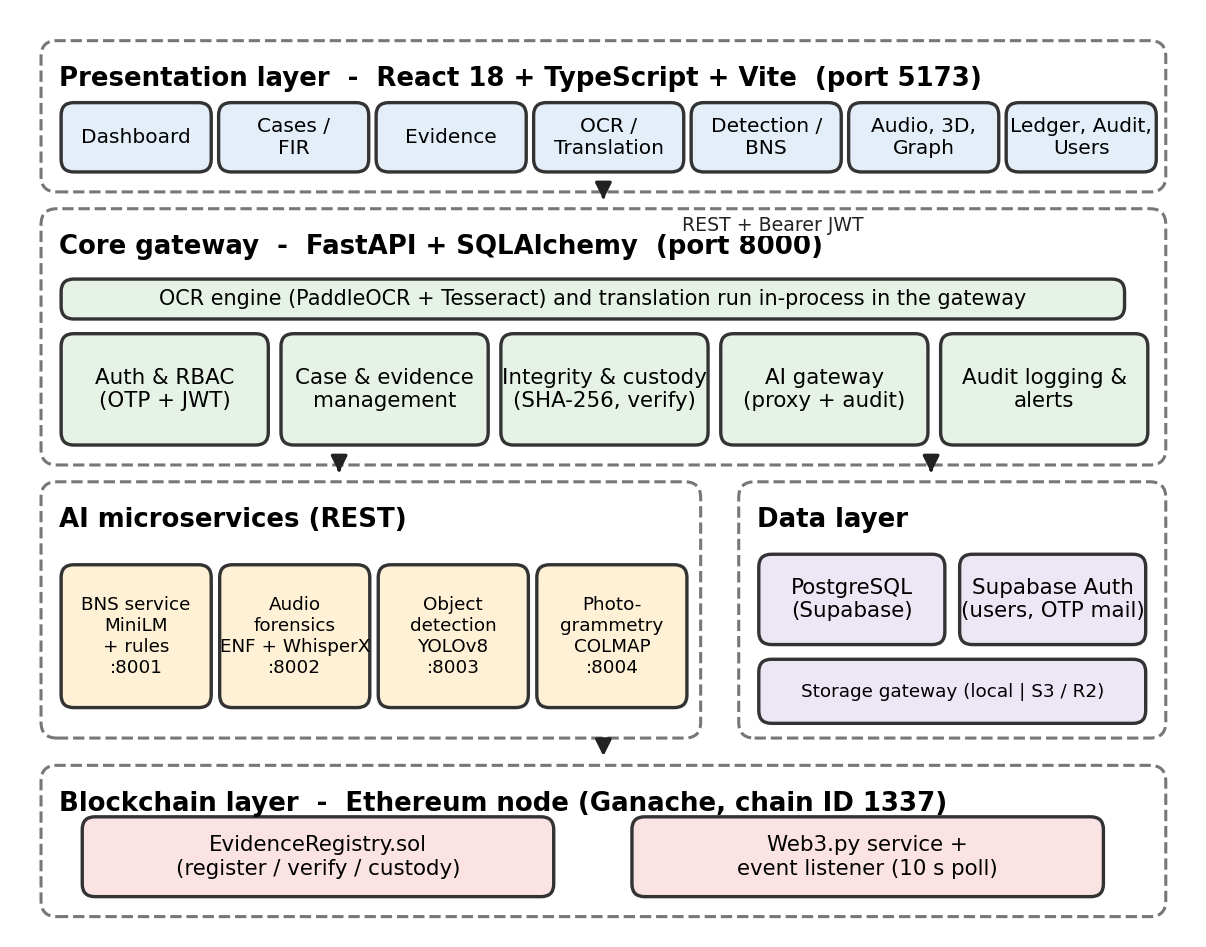
\includegraphics[width=14.8cm]{fig_architecture.png}
\caption{High-level architecture of Secure Audit}
\end{figure}

The responsibilities of the components are summarised in Table 7.

{\footnotesize
\setlength{\tabcolsep}{3pt}
\renewcommand{\arraystretch}{1.15}
\begin{longtable}{|>{\raggedright\arraybackslash}p{3.79cm}|>{\raggedright\arraybackslash}p{1.42cm}|>{\raggedright\arraybackslash}p{8.99cm}|}
\caption{System components and responsibilities}\\
\hline
\rowcolor{headfill}\textbf{Component} & \textbf{Port} & \textbf{Responsibility} \\ \hline
\endfirsthead
\hline
\rowcolor{headfill}\textbf{Component} & \textbf{Port} & \textbf{Responsibility} \\ \hline
\endhead
\hline \endfoot
Frontend (Vite dev server) & 5173 & User interface, session handling, calls to the gateway with a Bearer token, visualisation of results (charts, graph, 3D model). \\ \hline
Core gateway (FastAPI) & 8000 & Authentication, RBAC, case and evidence management, SHA-256 hashing, storage gateway, blockchain service, audit logging, alerts, OCR and translation, proxying to AI services. \\ \hline
BNS service & 8001 & Sentence-embedding retrieval and statutory element scoring of FIR text; returns ranked BNS sections with explanations. \\ \hline
Audio forensics service & 8002 & ENF analysis, splice and silence detection, transcription, diarization, keyword search and tamper assessment. \\ \hline
Object detection service & 8003 & YOLOv8 inference on images and videos; returns detections and annotated outputs. \\ \hline
Photogrammetry service & 8004 & Asynchronous video-to-3D jobs: frame extraction and selection, COLMAP, Open3D meshing and GLB export, evaluation metrics. \\ \hline
PostgreSQL / Supabase & --- & Relational storage of users, cases, evidence metadata, custody, audit and analysis results; identity through Supabase Auth. \\ \hline
Storage gateway & --- & Provider-agnostic, write-once evidence store (local disk or S3-compatible object storage). \\ \hline
Ethereum node and EvidenceRegistry & 8545 & Tamper-evident registry of evidence digests and custody events. \\ \hline
\end{longtable}
}

The gateway is the only component that touches the evidence store and the blockchain. The front end never accesses storage or the contract directly, which keeps authorisation and auditing in one place. A background thread in the gateway polls the contract for new events every 10 seconds (configurable) and mirrors them into the database.

\section{Decomposition Description}
Functionally, the platform is organised into six modules (Figure 2). Each module maps to a group of gateway routes and front-end pages.

\begin{figure}[htbp]
\centering
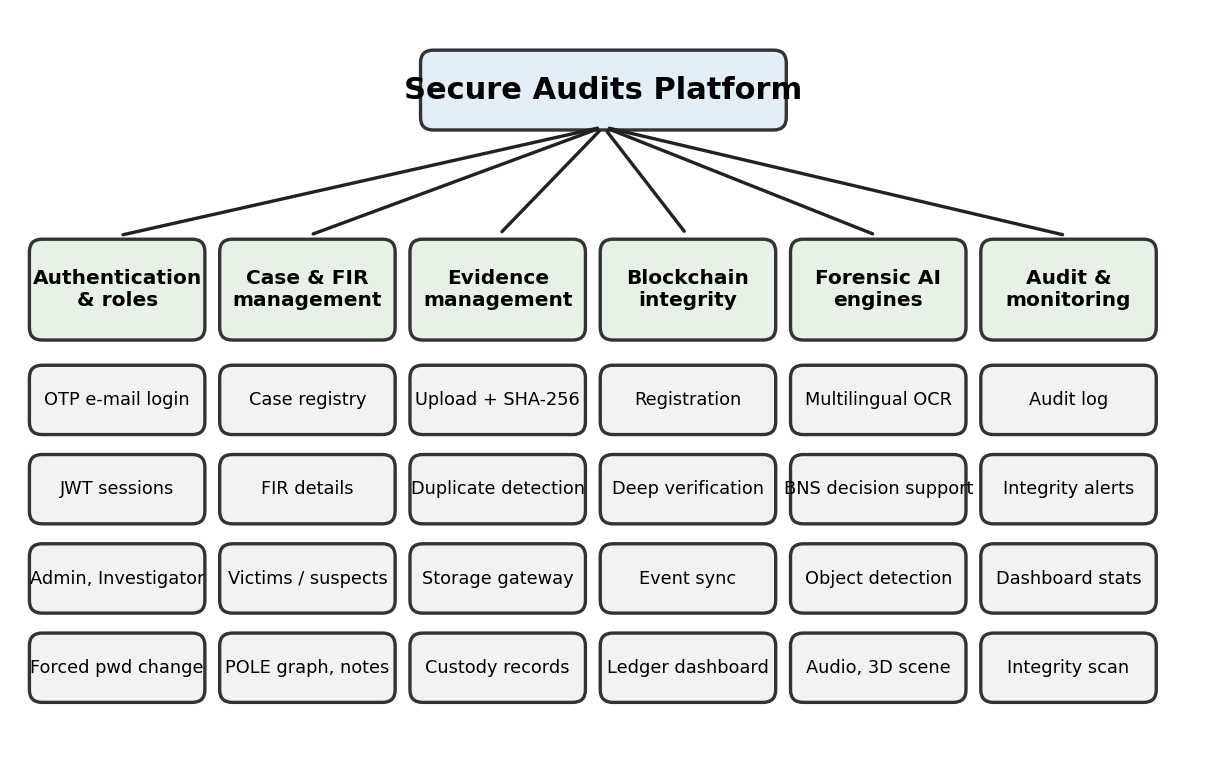
\includegraphics[width=15.0cm]{fig_decomposition.png}
\caption{Functional decomposition of Secure Audit}
\end{figure}

\section{Data Flow Design}
Figure 3 shows the context-level data flow. Users submit login, case, evidence and analysis requests to the gateway. The gateway verifies identity with Supabase Auth, stores metadata and audit rows in PostgreSQL, writes evidence bytes through the storage gateway, registers digests on the blockchain, and sends evidence to AI services for analysis. Results and integrity verdicts return to the user.

\begin{figure}[htbp]
\centering
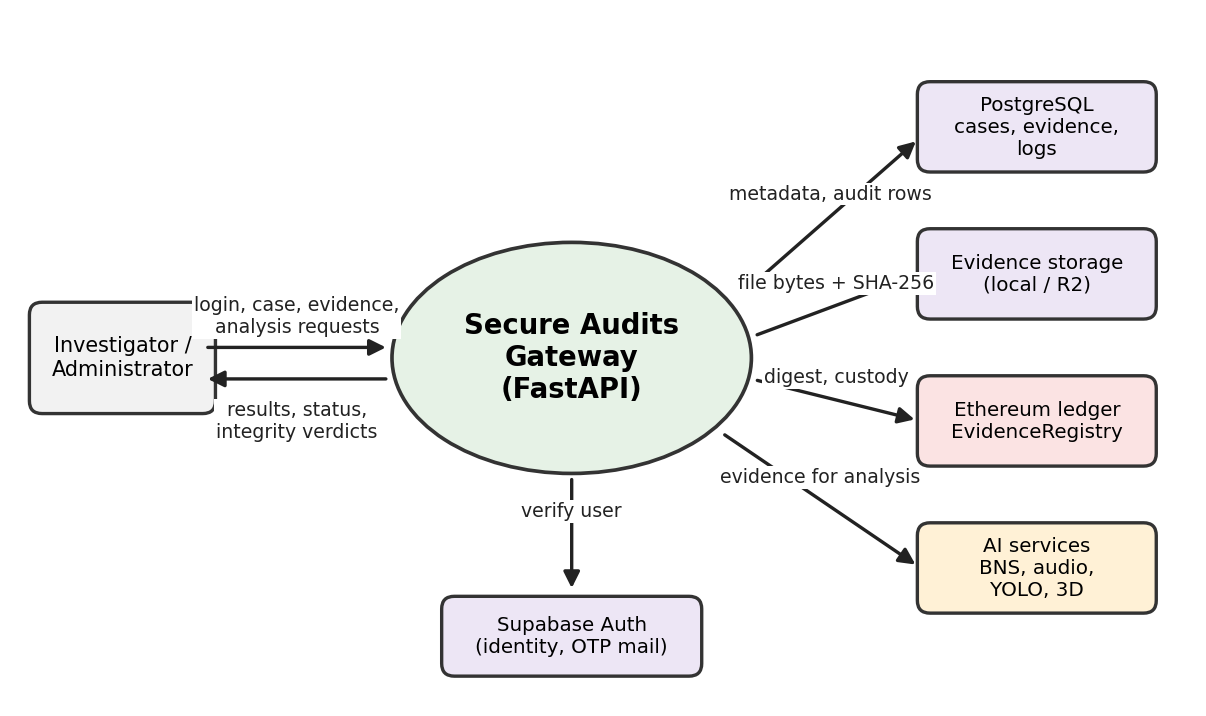
\includegraphics[width=14.5cm]{fig_dfd.png}
\caption{Data flow diagram (context level)}
\end{figure}

\section{Use Case Diagram}
Figure 4 shows the main use cases. Investigators manage their cases, upload and verify evidence, run analyses and review the audit trail. Administrators can perform the same functions across all cases and additionally manage users, run blockchain integrity scans and redeploy the ledger when required. The Ethereum ledger and the AI services appear as external systems.

\begin{figure}[htbp]
\centering
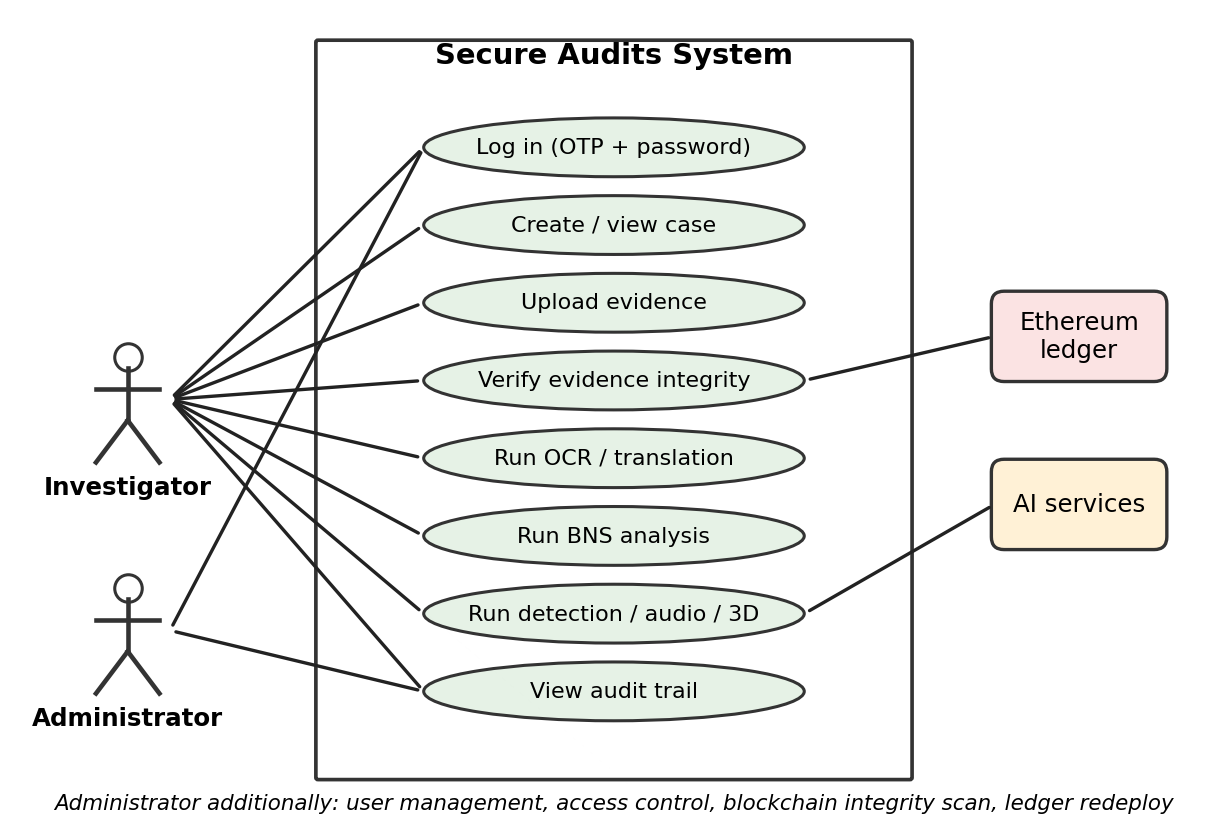
\includegraphics[width=14.0cm]{fig_usecase.png}
\caption{Use case diagram}
\end{figure}

\section{System Workflow}
The typical investigation workflow is shown in Figure 5. After login, the investigator creates a case and uploads evidence; the upload hashes, stores and anchors each file. Integrity can be verified at any time. Analyses are then run on verified evidence, results are reviewed and, where appropriate, stored, and every step is written to the audit log and custody trail.

\begin{figure}[htbp]
\centering
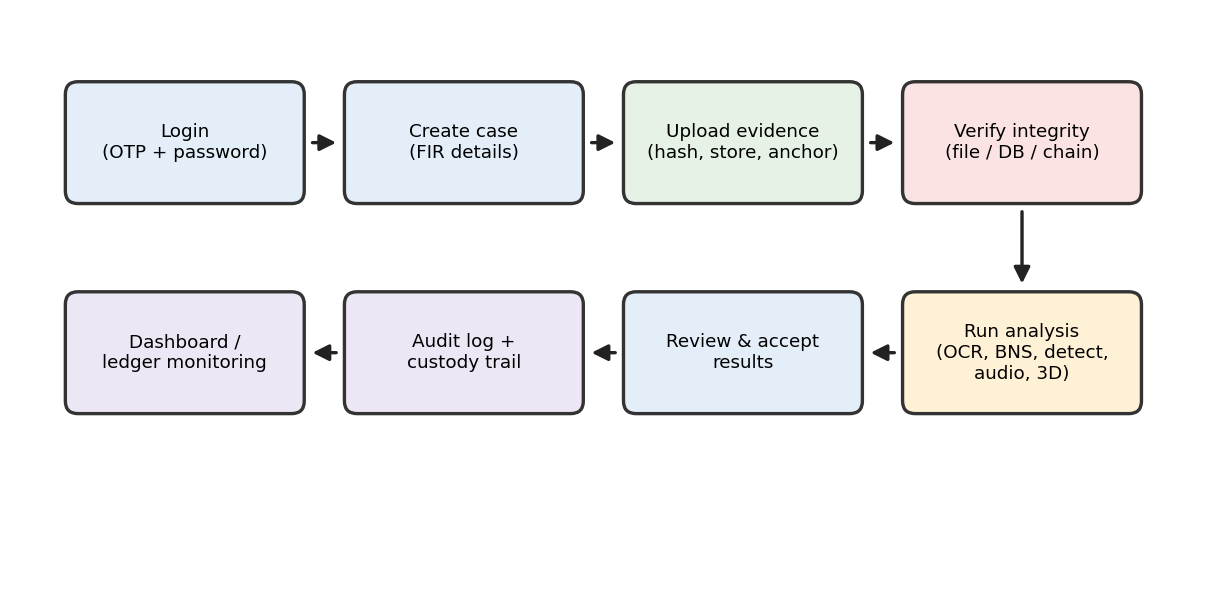
\includegraphics[width=15.0cm]{fig_workflow.png}
\caption{Investigation workflow in Secure Audit}
\end{figure}

\subsection{Evidence upload and registration}
Figure 6 shows the sequence for \code{POST /\allowbreak{}evidence/\allowbreak{}upload}. The gateway checks the caller's permission and case access, validates the file, computes SHA-256 and rejects a duplicate in the same case with HTTP 409 (the same file in another case is accepted but flagged in the audit log). The file is written through the storage gateway, the evidence row and a CREATED custody record are flushed, and the digest is registered on the blockchain. Only after a mined receipt is obtained are the receipt fields, the REGISTERED custody record and blockchain log committed. If registration fails, the transaction is rolled back, the stored file is discarded where the provider permits it, a failure is audited and the user receives HTTP 503, so no evidence row exists without an on-chain anchor.

\begin{figure}[htbp]
\centering
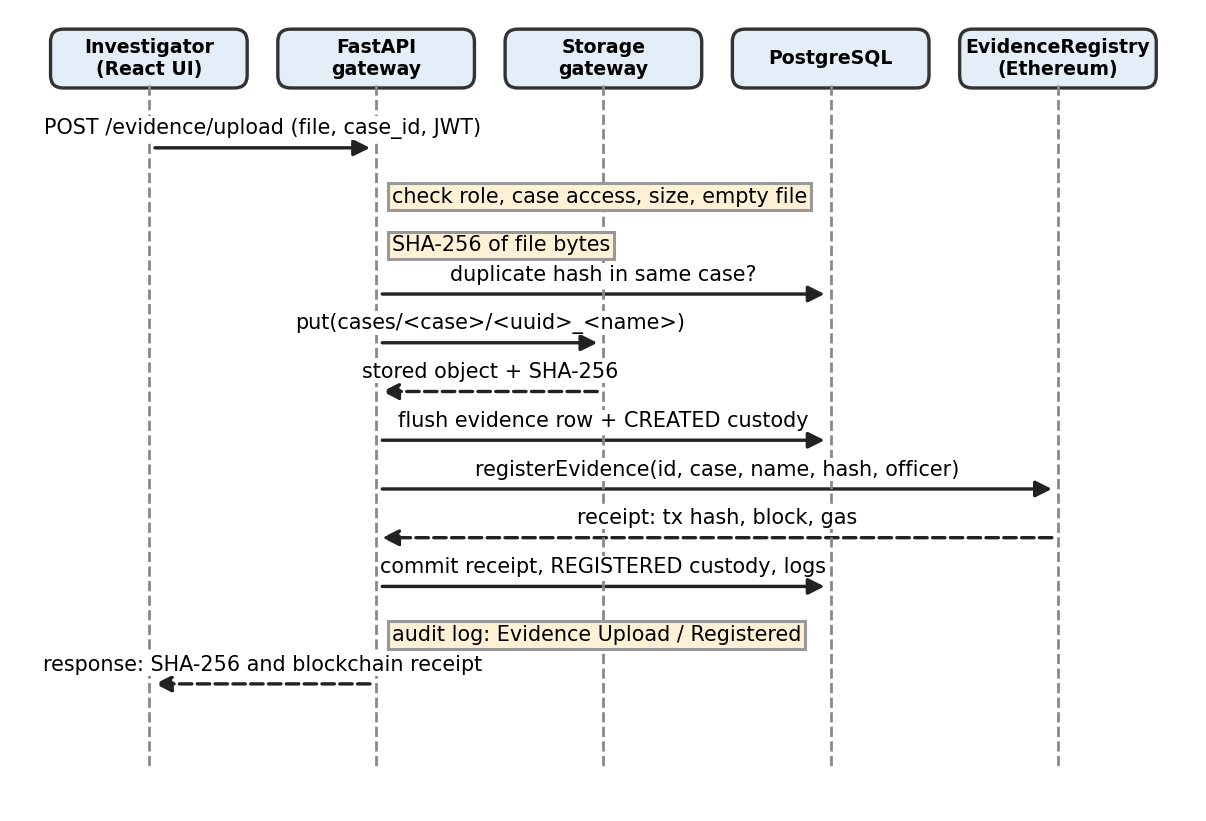
\includegraphics[width=15.0cm]{fig_seq_upload.png}
\caption{Sequence diagram of evidence upload and registration}
\end{figure}

\subsection{Evidence verification and retrieval}
Verification (\code{POST /\allowbreak{}evidence/\allowbreak{}\{id\}/\allowbreak{}verify}, deep mode by default) streams the stored object, computes its SHA-256 independently of stored metadata, reads the registered record from the contract and compares file, database and blockchain digests (Figure 7). Retrieval through \code{GET /\allowbreak{}evidence/\allowbreak{}\{id\}/\allowbreak{}download} is authenticated, checks case access, and records a DOWNLOADED custody event.

\begin{figure}[htbp]
\centering
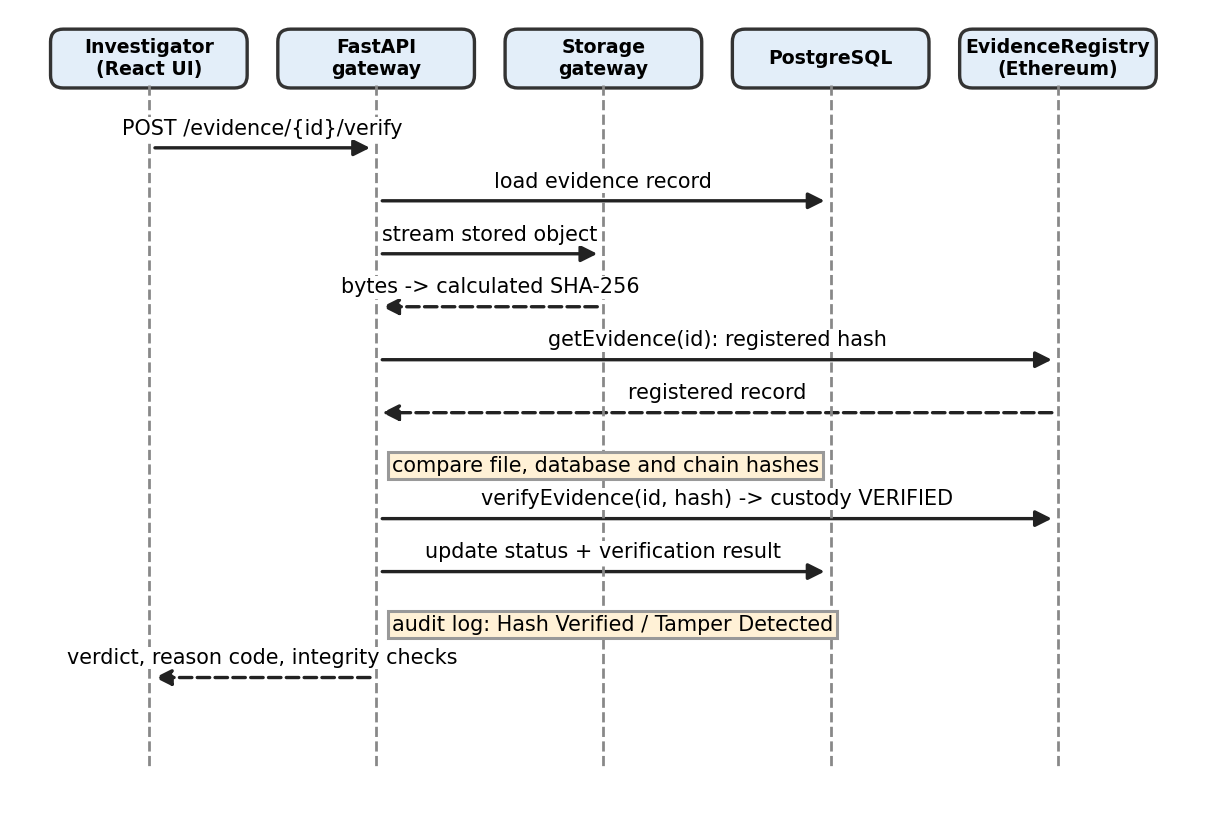
\includegraphics[width=15.0cm]{fig_seq_verify.png}
\caption{Sequence diagram of evidence verification}
\end{figure}

\section{Database Design}
Secure Audit uses a relational PostgreSQL schema accessed through SQLAlchemy models (\code{backend/\allowbreak{}models.py}) and defined in \code{schema.sql}. Eleven tables hold users, cases, evidence, custody, blockchain logs, audit logs, OTP tokens and analysis results (Figure 8). Primary keys are UUIDs; evidence-related foreign keys use \code{ON DELETE RESTRICT}, so cases and evidence that have dependent records cannot be removed silently. Flexible structures such as victims, suspects, detection predictions, OCR page metadata and BNS sections are stored as JSONB.

\begin{figure}[htbp]
\centering
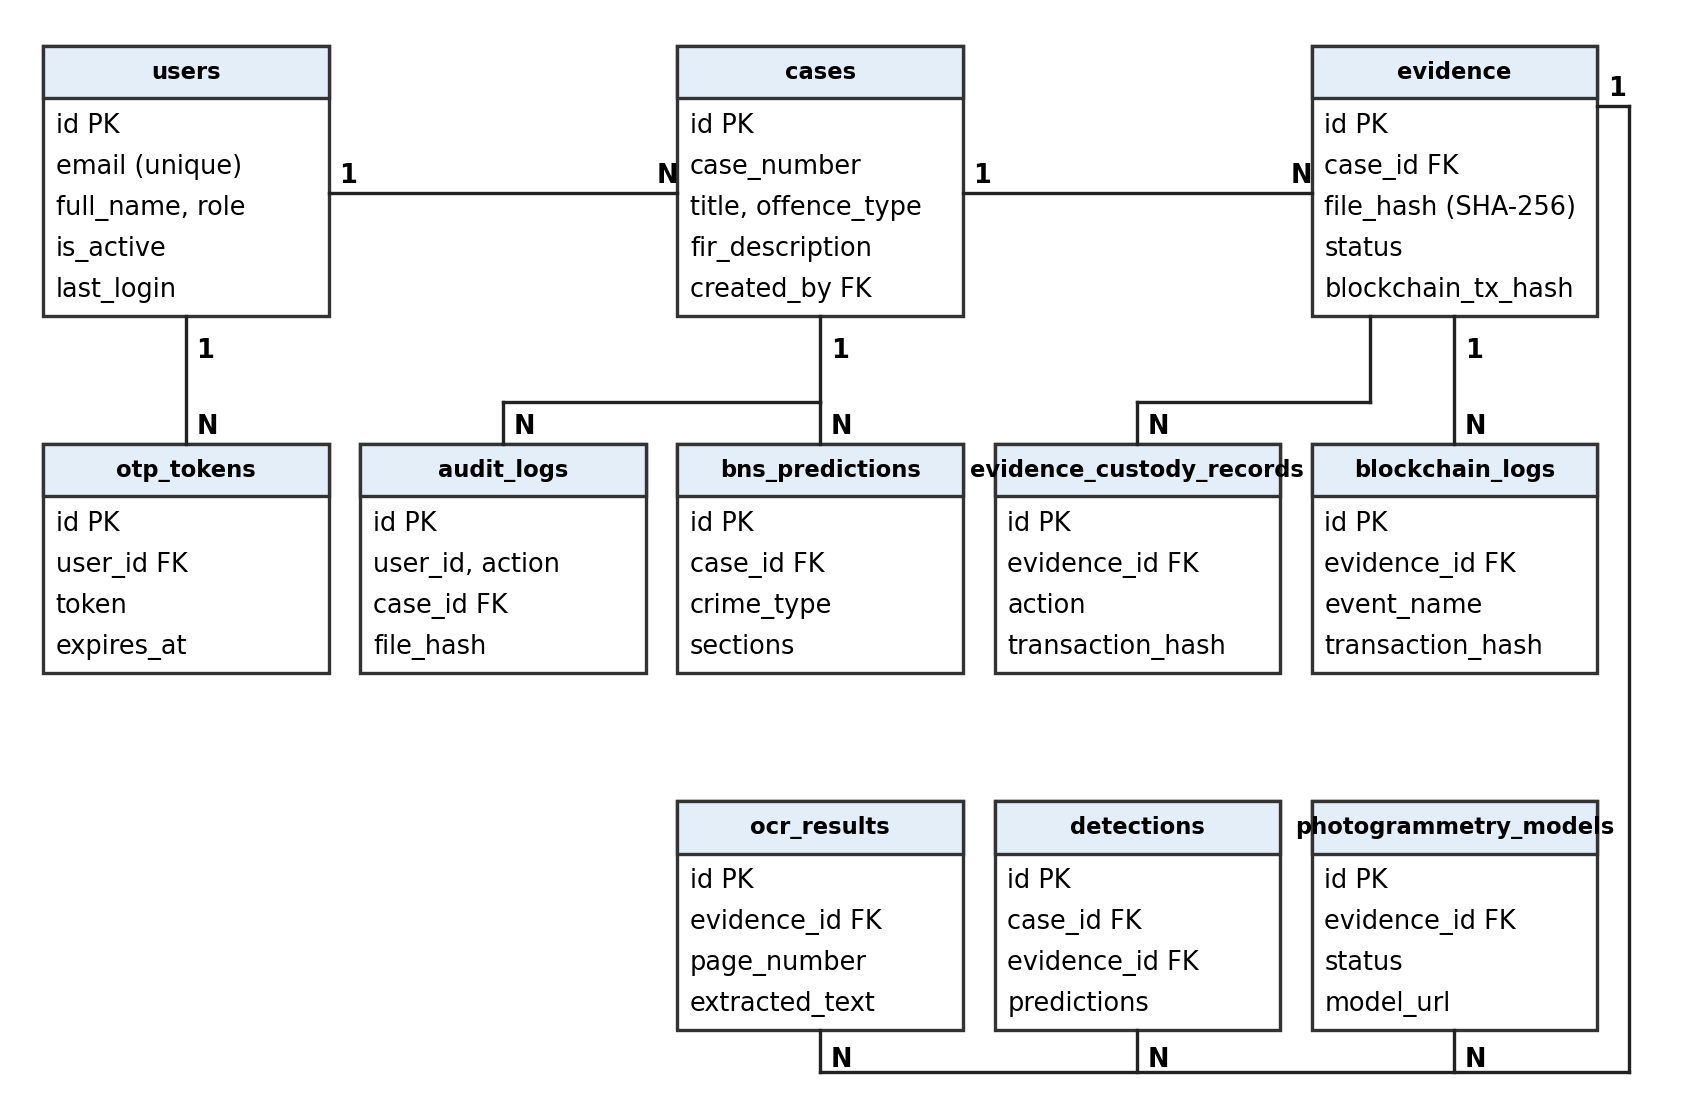
\includegraphics[width=15.4cm]{fig_er.png}
\caption{Entity--relationship diagram}
\end{figure}

{\footnotesize
\setlength{\tabcolsep}{3pt}
\renewcommand{\arraystretch}{1.15}
\begin{longtable}{|>{\raggedright\arraybackslash}p{3.22cm}|>{\raggedright\arraybackslash}p{3.98cm}|>{\raggedright\arraybackslash}p{7.01cm}|}
\caption{Database tables}\\
\hline
\rowcolor{headfill}\textbf{Table} & \textbf{Purpose} & \textbf{Key columns} \\ \hline
\endfirsthead
\hline
\rowcolor{headfill}\textbf{Table} & \textbf{Purpose} & \textbf{Key columns} \\ \hline
\endhead
\hline \endfoot
users & Officers synchronised from Supabase Auth & id, email (unique), full\_name, role, department, badge\_number, clearance\_level, is\_active, can\_create\_case, last\_login \\ \hline
cases & Case registry and FIR details & id, case\_number (unique), title, offence\_type, fir\_description, fir\_language, complainant, victims, suspects, incident date/time/location, created\_by, is\_archived \\ \hline
evidence & Evidence metadata, integrity state and blockchain receipt & id, case\_id, evidence\_type, file\_url, file\_hash, file\_name, file\_size, mime\_type, uploaded\_by, status, chain\_of\_custody\_status, blockchain\_tx\_hash (unique), block number/hash, contract address, gas used, chain ID, last\_verification\_result/reason \\ \hline
evidence\_custody\_records & Chain-of-custody events & evidence\_id, officer\_id, action, occurred\_at, transaction\_hash, block\_number, source (blockchain or database), details \\ \hline
blockchain\_logs & Mirrored contract events & evidence\_id, event\_name, transaction\_hash, block\_number, payload \\ \hline
audit\_logs & Application audit trail & user\_id, action, case\_id, file\_hash, metadata, created\_at \\ \hline
otp\_tokens & Single-use login codes & user\_id, token, expires\_at, used \\ \hline
detections & Object-detection results & case\_id, evidence\_id, image\_url, predictions (JSONB) \\ \hline
ocr\_results & Page-wise OCR output (one row per evidence page) & evidence\_id, page\_number, extracted\_text, language, confidence, detected\_languages, ocr\_metadata \\ \hline
bns\_predictions & Accepted BNS suggestions & case\_id, crime\_type, sections (JSONB), fir\_text \\ \hline
photogrammetry\_models & 3D reconstruction jobs & case\_id, evidence\_id, status (Pending, Processing, Completed, Failed), current\_step, model\_url, point\_cloud\_url, frame\_count, error\_message \\ \hline
\end{longtable}
}

Personal notes are kept in a Supabase \code{personal\_\allowbreak{}notes} table accessed through the gateway, and user identities and passwords are held by Supabase Auth rather than in the application tables.

\section{Evidence Storage Architecture}
Evidence bytes are not stored in the database. The \code{StorageProvider} abstraction in \code{backend/\allowbreak{}services/\allowbreak{}storage\_\allowbreak{}gateway.py} offers \code{put}, \code{get}, \code{stat} and \code{exists}, and deliberately has no delete or overwrite operation. Two providers are implemented and selected with \code{STORAGE\_\allowbreak{}BACKEND} (Figure 9).

\begin{figure}[htbp]
\centering
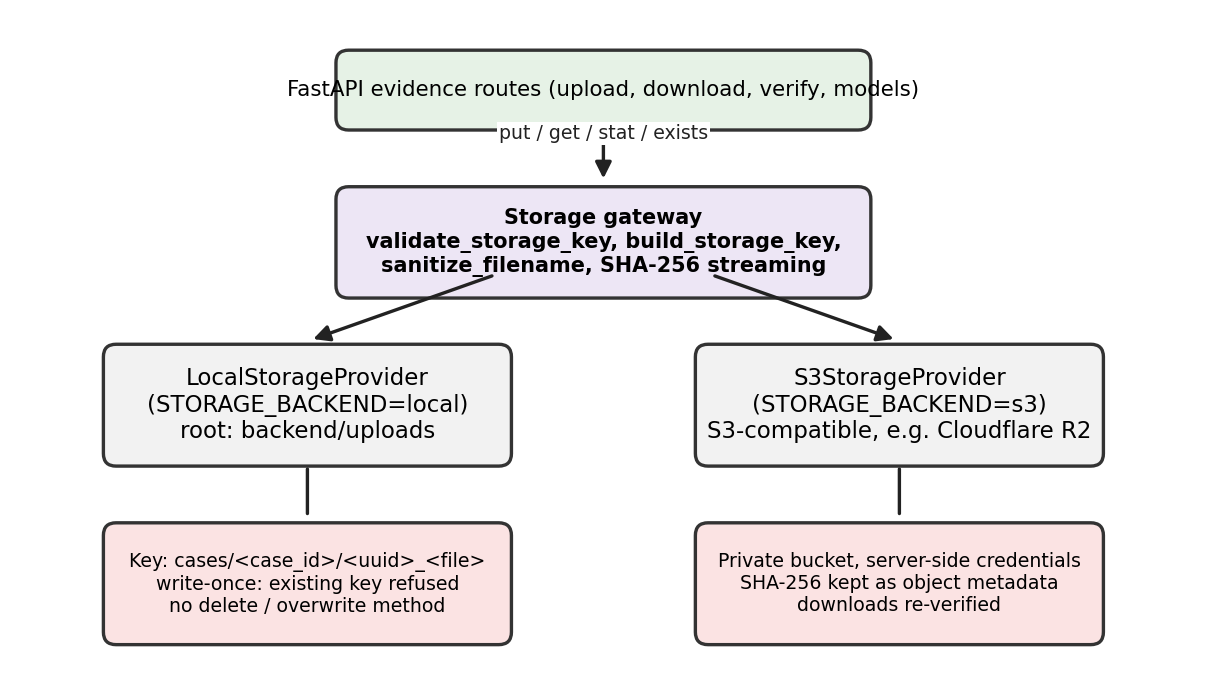
\includegraphics[width=14.0cm]{fig_storage.png}
\caption{Evidence storage architecture}
\end{figure}

\begin{itemize}
  \item \textbf{Key scheme:} \code{cases/\allowbreak{}\textless{}case\_\allowbreak{}uuid\textgreater{}/\allowbreak{}\textless{}file\_\allowbreak{}uuid\textgreater{}\_\allowbreak{}\textless{}sanitised\_\allowbreak{}name\textgreater{}}; 3D models are stored under \code{models/\allowbreak{}\textless{}case\_\allowbreak{}uuid\textgreater{}/\allowbreak{}\textless{}job\_\allowbreak{}uuid\textgreater{}\_\allowbreak{}model.\textless{}glb\textbar{}ply\textgreater{}}. Filenames are stripped of directory markers and unsafe characters.
  \item \textbf{Write-once semantics:} \code{put()} refuses an existing key (\code{KeyAlreadyExistsError}), so an exhibit cannot be replaced after acquisition.
  \item \textbf{Path-traversal defence:} \code{validate\_\allowbreak{}storage\_\allowbreak{}key} rejects absolute paths, drive letters and \code{.}/\code{..} segments (\code{PathTraversalError}).
  \item \textbf{Stream hashing:} the SHA-256 of the stored bytes is calculated during storage; the upload route compares it with the hash computed from the upload and rejects a mismatch.
  \item \textbf{S3-compatible provider:} works with AWS S3, MinIO and Cloudflare R2, uses private objects and optional server-side encryption, keeps the SHA-256 as object metadata and maps provider failures to explicit errors (permission denied, unavailable, not found, integrity error).
  \item \textbf{Local provider:} rooted at \code{backend/\allowbreak{}uploads} for development and air-gapped use.
  \item \textbf{Records that predate the gateway:} older evidence rows referencing local or Supabase Storage URLs are still resolved for download and verification.
\end{itemize}

Because the database keeps only the key (\code{file\_\allowbreak{}url}) and the digest, the database and the object store are connected by the evidence identifier and the SHA-256, which the verification procedure checks against the blockchain.

\section{Security and Access Control}
\subsection{Authentication}
Login is a two-step process. In step one, \code{POST /\allowbreak{}auth/\allowbreak{}send-otp} checks that the e-mail belongs to an active user in Supabase, generates a six-digit OTP valid for five minutes and delivers it by SMTP; the OTP is stored in \code{otp\_\allowbreak{}tokens} only after successful delivery. In step two, \code{POST /\allowbreak{}auth/\allowbreak{}verify-otp} validates the password with Supabase Auth together with the OTP and issues a JWT signed with HS256 and a 24-hour expiry carrying the user id, e-mail, role and name. The front end keeps the token and attaches it as a Bearer header on every request; a 401 response, or a 403 for a deactivated account, clears the session. Users created or reset by an administrator carry a \code{must\_\allowbreak{}change\_\allowbreak{}password} flag, and the front end routes them to a forced password-change page before any other page is accessible.

\subsection{Authorisation}
Every protected route resolves the caller from the JWT and calls \code{has\_\allowbreak{}permission} for the required permission (Table 4). Case-bound routes call \code{check\_\allowbreak{}case\_\allowbreak{}access}: administrators see all cases, whereas an investigator is denied (HTTP 403) access to a case created by another user. Evidence and analysis routes load the evidence through the same ownership check, and administrator-only operations (user management, blockchain integrity scan, ledger redeploy) call \code{require\_\allowbreak{}admin}, which also audits unauthorised attempts.

\subsection{Additional safeguards}
\begin{itemize}
  \item Input validation: UUID parsing for identifiers, length limits on text fields, empty-file and maximum-size checks.
  \item Configurable CORS origins and an optional trusted-proxy setting for client IP recording.
  \item Secrets, keys and credentials are read only from environment variables; none are stored in source code.
  \item The blockchain signing key is held by the gateway; the contract restricts state-changing calls to registrar accounts.
  \item Evidence files are served only through authenticated gateway routes.
\end{itemize}

\section{Evidence Integrity and Auditability}
\subsection{EvidenceRegistry smart contract}
\code{EvidenceRegistry.sol} (Solidity 0.8.28) stores, for each evidence identifier, the case ID, file name, SHA-256 string (exactly 64 hex characters), uploader and block timestamp, and keeps an append-only custody history. Registration, verification and custody-recording functions are restricted to authorised registrar accounts managed by the contract owner; \code{registerEvidence} rejects an identifier that already exists. Custody actions are limited to REGISTERED, VERIFIED and TRANSFERRED. The contract emits \code{EvidenceRegistered}, \code{EvidenceVerified}, \code{EvidenceTampered}, \code{CustodyTransferred}, \code{RegistrarUpdated} and \code{OwnershipTransferred} events. Read-only functions (\code{getEvidence}, \code{checkEvidence}, \code{isRegistered}, \code{getCustodyHistory}, \code{getCustodyCount}) allow verification without cost.

\subsection{Verification outcomes}
The outcome of verification is expressed as one of four evidence states, stored in \code{evidence.status}, together with a machine-readable reason (Table 9). A failed attempt caused by an outage is stored separately in \code{last\_\allowbreak{}verification\_\allowbreak{}result} as ``Verification Failed'', so that an unreachable node or storage can never overwrite the real integrity state of an exhibit.

{\footnotesize
\setlength{\tabcolsep}{3pt}
\renewcommand{\arraystretch}{1.15}
\begin{longtable}{|>{\raggedright\arraybackslash}p{3.60cm}|>{\raggedright\arraybackslash}p{4.45cm}|>{\raggedright\arraybackslash}p{6.15cm}|}
\caption{Integrity states and reason codes}\\
\hline
\rowcolor{headfill}\textbf{State / result} & \textbf{Reason code} & \textbf{Meaning} \\ \hline
\endfirsthead
\hline
\rowcolor{headfill}\textbf{State / result} & \textbf{Reason code} & \textbf{Meaning} \\ \hline
\endhead
\hline \endfoot
Verified & HASH\_MATCH & Stored file matches the registered blockchain hash. \\ \hline
Tampered & HASH\_MISMATCH, BYTE\_HASH\_MISMATCH & Calculated SHA-256 of the stored bytes differs from the registered hash. \\ \hline
Missing & EVIDENCE\_MISSING & The object no longer exists in storage. \\ \hline
Unregistered & NOT\_REGISTERED & The evidence has no registration on the blockchain. \\ \hline
Verified with warning & DATABASE\_MISMATCH & The database hash differs from the blockchain hash although the file matches the chain. \\ \hline
Verification Failed (attempt only) & BLOCKCHAIN\_UNAVAILABLE, STORAGE\_UNAVAILABLE, OBJECT\_UNREADABLE, TRANSACTION\_FAILED & Integrity could not be checked; evidence state is unchanged. \\ \hline
\end{longtable}
}

\begin{figure}[htbp]
\centering
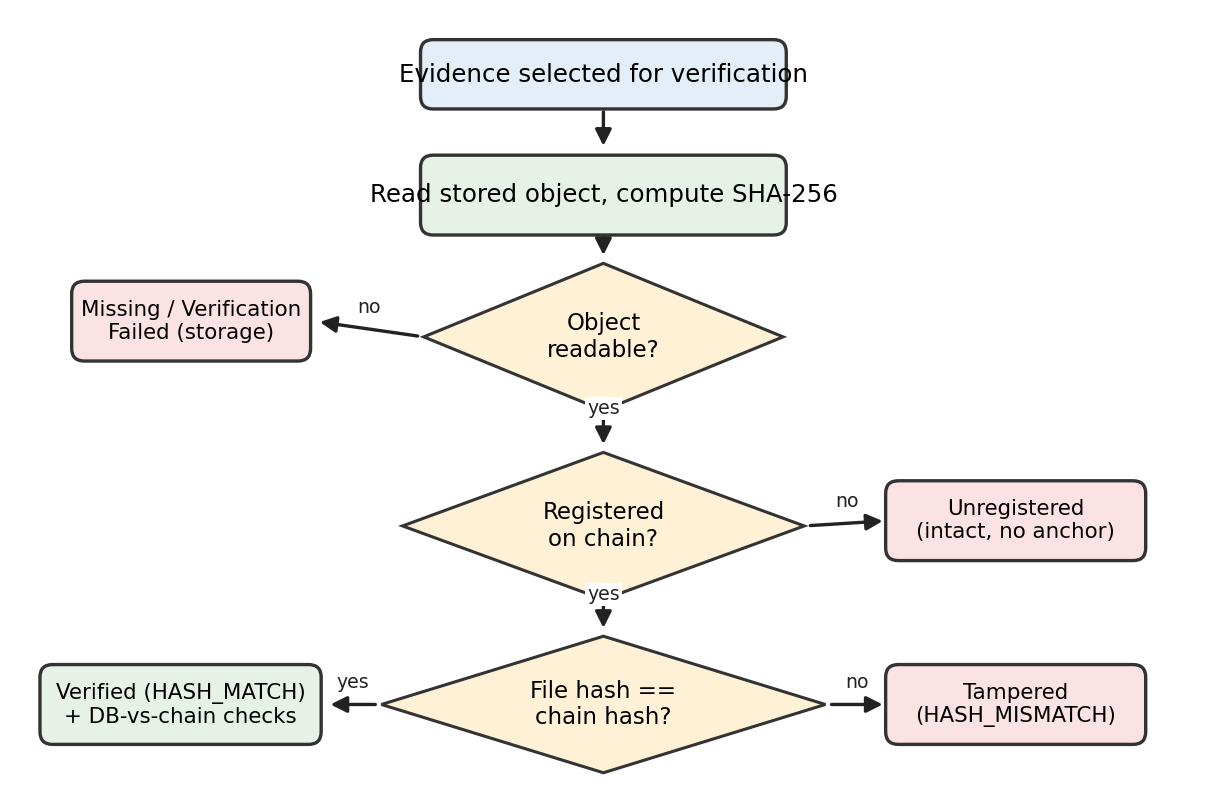
\includegraphics[width=13.5cm]{fig_verify_flow.png}
\caption{Evidence integrity decision flow}
\end{figure}

In addition to the file check, \code{integrity\_\allowbreak{}checks} evaluates consistency of the database record with the chain: valid hash format, complete receipt metadata, database hash equals chain hash, file name and case unchanged, registration transaction present, block and contract match, and uniqueness of the hash. The summary is Consistent, Warning or Inconsistent, depending on whether any failed check is critical.

\subsection{Chain of custody and event synchronisation}
Custody is recorded in two ways. On-chain events (REGISTERED, VERIFIED, TRANSFERRED) are enforced by the contract. Off-chain events (CREATED, VIEWED, DOWNLOADED, METADATA\_MODIFIED) are written to \code{evidence\_\allowbreak{}custody\_\allowbreak{}records} with \code{source = database}. A listener thread in the gateway reads contract events since the last processed block, avoids duplicate rows and mirrors them into \code{evidence\_\allowbreak{}custody\_\allowbreak{}records} and \code{blockchain\_\allowbreak{}logs}, so events created outside the API are also reflected in the database.

\subsection{Audit logging}
Audit entries record the user, action, case, file hash, metadata (including client IP and result) and a timestamp. Defined actions include Evidence Upload, Evidence Registered, Hash Verified, Tamper Detected, Evidence Missing, Database Hash Mismatch, Duplicate Evidence Hash Detected, Evidence Downloaded, Evidence Custody Transferred, YOLO Scan, BNS Section Prediction, Audio Forensics Analysis and OCR runs. Actions that signal a problem (for example tampering or an unauthorised blockchain action) are shown with Warning status and failures with Failed status in the audit page and dashboard. The application treats the audit table as append-only and does not expose update or delete routes for it.

\chapter{Implementation}
This chapter describes how each module of Secure Audit is implemented. The core gateway is a single FastAPI application (\code{backend/\allowbreak{}app.py}) supported by service modules; the four analysis services are independent FastAPI applications.

\section{Frontend}
The frontend (\code{audit-frontend}) is a React 18 and TypeScript application built with Vite. \code{App.tsx} defines the routes; a \code{ProtectedRoute} wrapper redirects unauthenticated users to the login page and users who must change their password to the forced password-change page. \code{AuthContext} stores the session token, and a single Axios client in \code{services/\allowbreak{}api.ts} attaches the Bearer token and handles 401 responses globally. Theme switching is provided by \code{ThemeContext}.

{\footnotesize
\setlength{\tabcolsep}{3pt}
\renewcommand{\arraystretch}{1.15}
\begin{longtable}{|>{\raggedright\arraybackslash}p{4.17cm}|>{\raggedright\arraybackslash}p{3.41cm}|>{\raggedright\arraybackslash}p{6.63cm}|}
\caption{Main frontend pages}\\
\hline
\rowcolor{headfill}\textbf{Route} & \textbf{Page} & \textbf{Function} \\ \hline
\endfirsthead
\hline
\rowcolor{headfill}\textbf{Route} & \textbf{Page} & \textbf{Function} \\ \hline
\endhead
\hline \endfoot
/login & AuthPage & Two-step OTP and password login \\ \hline
/dashboard & Dashboard & Case and evidence statistics and recent activity \\ \hline
/cases, /cases/new, /cases/:id & Cases, CreateCase, CaseDetail & Case list, FIR entry and case workspace with evidence \\ \hline
/evidence & EvidencePage & Upload, hash display, verification, download, custody and blockchain details \\ \hline
/ocr & OCRPage & Language selection, page-wise text, original and translated views, copy and download \\ \hline
/detection & DetectionPage & Detection overlay with percentage-based bounding boxes \\ \hline
/bns & BNSPage & FIR text entry, ranked sections with explanations, accept and store \\ \hline
/audio & AudioForensicsPage & ENF graph, speaker segments, transcript, keywords and printable report \\ \hline
/photo3d & Photo3DPage & Reconstruction trigger, step progress and Three.js model viewer \\ \hline
/graph, /cases/:id/graph & GraphPage & POLE relationship graph (React Flow) \\ \hline
/personal & PersonalPage & Personal notes and sketches \\ \hline
/audit & AuditPage & Filtered audit log with status \\ \hline
/blockchain & BlockchainDashboard & Network status, ledger, transactions, custody and integrity scan \\ \hline
/users, /profile & UsersPage, ProfilePage & User administration and personal profile \\ \hline
\end{longtable}
}

\section{Core Backend and API}
The gateway exposes REST endpoints grouped as shown in Table 11. Startup hooks apply additive, idempotent schema statements for blockchain and OCR columns and start the blockchain event listener.

{\footnotesize
\setlength{\tabcolsep}{3pt}
\renewcommand{\arraystretch}{1.15}
\begin{longtable}{|>{\raggedright\arraybackslash}p{2.46cm}|>{\raggedright\arraybackslash}p{7.01cm}|>{\raggedright\arraybackslash}p{4.73cm}|}
\caption{Core gateway endpoint groups}\\
\hline
\rowcolor{headfill}\textbf{Group} & \textbf{Representative endpoints} & \textbf{Description} \\ \hline
\endfirsthead
\hline
\rowcolor{headfill}\textbf{Group} & \textbf{Representative endpoints} & \textbf{Description} \\ \hline
\endhead
\hline \endfoot
Authentication & POST /auth/send-otp, /auth/verify-otp, /auth/change-password, /auth/reset-password; GET /auth/me & OTP login, JWT issue, password management \\ \hline
Cases & POST /cases; GET /cases, /cases/stats, /cases/\{id\}, /cases/\{id\}/graph & Case registry, statistics and POLE graph data \\ \hline
Evidence & POST /evidence/upload; GET /evidence, /evidence/\{id\}/download; POST /evidence/\{id\}/verify; PATCH /evidence/\{id\}; POST /evidence/\{id\}/custody/transfer & Upload, listing, download, verification, metadata and custody \\ \hline
Blockchain & GET /blockchain/status, /network, /ledger, /dashboard, /history/\{id\}, /transaction/\{tx\}; POST /blockchain/register, /verify, /integrity-scan & Ledger access and integrity operations \\ \hline
AI gateway & POST /ai/detect, /ai/ocr/\{id\}, /ai/audio/analyze, /bns/predict, /bns/store; GET /ai/detect/case/\{id\}, /ai/bns/case/\{id\}, /bns/case/\{id\}, /ocr/search & Authorised proxying to analysis services and result storage \\ \hline
Photogrammetry & POST /photogrammetry/trigger/\{case\_id\}; GET /photogrammetry/status/\{case\_id\}, /evaluation/\{job\_id\}, /comparison, /model/\{job\_id\}/\{fmt\} & 3D reconstruction jobs and artefacts \\ \hline
Audit and notes & GET /audit; GET/POST/PATCH /notes & Audit retrieval and personal notes \\ \hline
Users (admin) & GET/POST /users; PATCH /users/\{id\}; POST /users/\{id\}/reset-access & User administration \\ \hline
System & GET /health; POST /admin/blockchain/redeploy & Health check and ledger redeploy \\ \hline
\end{longtable}
}

\section{Case and Evidence Management Module}
Case creation assigns a case number and stores FIR details, victims, suspects and incident data; the case list is filtered by ownership for investigators. The evidence module implements the upload pipeline of Section 4.5.1: validation, streaming-safe size limit (default 200 MB, \code{MAX\_\allowbreak{}UPLOAD\_\allowbreak{}MB}), SHA-256, duplicate check, storage-gateway write, transactional database and blockchain registration, custody records and audit entries. Download re-hashes the bytes being served and records the result. Evidence metadata updates are audited as METADATA\_MODIFIED custody events, and evidence is never deleted through the API.

\section{Blockchain Integration Module}
\code{EvidenceBlockchainService} (\code{services/\allowbreak{}blockchain\_\allowbreak{}service.py}) is the only code that talks to the node. It builds a Web3.py connection from \code{ETHEREUM\_\allowbreak{}RPC\_\allowbreak{}URL}, loads the contract ABI and address, signs transactions with the configured key, retries transient failures, waits for receipts (and optionally a number of confirmations), and translates reverts into typed errors (\code{BlockchainUnavailable}, \code{BlockchainTransactionError}). It exposes register, verify, read-registration, receipt lookup, transaction details, custody history, recent blocks and event-since queries. The contract is compiled and deployed with Hardhat (\code{blockchain/\allowbreak{}scripts/\allowbreak{}deploy.js}), and a local Ganache node (chain ID 1337) provides the network; the deployment record contains only the contract address, transaction hash, chain ID and time. The gateway can redeploy the contract through an administrator-only route when a development ledger has been reset.

\section{Multilingual OCR and Translation Module}
OCR runs inside the gateway (\code{services/\allowbreak{}ocr\_\allowbreak{}service.py}, \code{ocr\_\allowbreak{}text.py}, \code{tesseract\_\allowbreak{}engine.py}). \code{POST /\allowbreak{}ai/\allowbreak{}ocr/\allowbreak{}\{evidence\_\allowbreak{}id\}} loads the evidence for the current user, applies file-size and page limits, runs the pipeline in Figure 11 and stores one row per page in \code{ocr\_\allowbreak{}results}; re-running OCR replaces the rows. The user may select a language or \code{auto}; supported languages are English, Hindi, Kannada, Telugu, Tamil and Malayalam, and an optional translation target can be requested.

\begin{figure}[htbp]
\centering
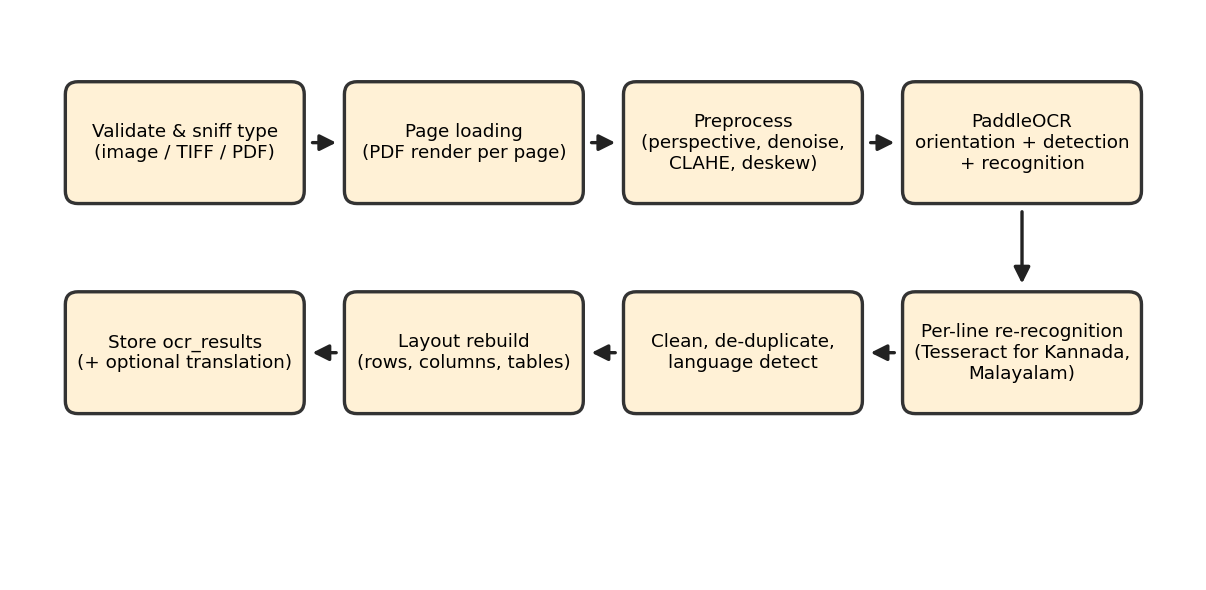
\includegraphics[width=15.0cm]{fig_ocr_pipeline.png}
\caption{Multilingual OCR pipeline}
\end{figure}

\begin{itemize}
  \item \textbf{Input handling:} file type is sniffed and validated (PNG, JPEG, WEBP, TIFF, BMP, GIF or PDF); PDFs are rendered page by page.
  \item \textbf{Preprocessing (applied only when needed):} perspective correction for photographed pages, downscaling of oversized images and upscaling with sharpening of low-resolution ones, edge-aware denoising, CLAHE contrast enhancement on the lightness channel for faded pages, and deskewing. Binarisation is deliberately avoided because the PaddleOCR models are trained on natural colour images.
  \item \textbf{Recognition:} PaddleOCR (PP-OCRv5 detection, orientation handling and recognisers) detects and recognises text lines. Lines are re-recognised with other candidate languages; Tesseract 5 with script-specific models reads Kannada and Malayalam lines (Malayalam has no PaddleOCR model), by stacking line crops into one image per language to avoid per-line process start-up.
  \item \textbf{Post-processing:} noise segments and duplicates are removed, mixed-script lines are labelled with per-script language detection, and layout is rebuilt by grouping boxes into rows and cells to preserve paragraphs, lists and tables.
  \item \textbf{Translation:} after OCR, text is translated paragraph by paragraph by language group through \code{deep-translator} providers (Google, then MyMemory) with caching and provider cool-down. The original OCR text is never replaced, failures are reported rather than raised, and the interface advises verification against the original.
\end{itemize}

Each page record stores text, language, confidence, detected languages and metadata (status, warnings, tables, line boxes, preprocessing steps and processing time). A search route (\code{/\allowbreak{}ocr/\allowbreak{}search}) queries stored text. OCR output is not forwarded automatically to the BNS module; the investigator reviews or edits the text before analysis.

\section{Object Detection Module}
The detection microservice (\code{best/\allowbreak{}app.py}) loads a fine-tuned YOLOv8 model through Ultralytics (falling back to the standard \code{yolov8n.pt} weights when the custom weights are absent). Its health endpoint reports the loaded class names, and the integration test expects six classes including pistol, knife, person and lying\_person. \code{POST /\allowbreak{}detect/\allowbreak{}image} decodes the image with OpenCV, runs inference at a default confidence of 0.25, returns label, confidence and bounding box for each object together with the SHA-256 of the input, and writes an annotated image with a UUID-based name. \code{POST /\allowbreak{}detect/\allowbreak{}video} processes a video frame by frame and returns an annotated video and per-class frequencies.

In the gateway, \code{POST /\allowbreak{}ai/\allowbreak{}detect} first loads the evidence, verifies the caller's case access and recomputes the file's SHA-256. If the stored hash and the current hash differ, detection is blocked with an integrity error. Otherwise the image is sent to the service, bounding boxes are converted to percentages of the image size so that the overlay scales with the displayed image, the result is stored in \code{detections}, and a ``YOLO Scan'' audit entry is written.

\section{BNS Decision Support Module}
The BNS service (\code{bns-backend}) classifies an FIR narrative against statutory profiles. Each profile is built from the section title, description, legal elements and keywords, and is embedded with the \code{all-MiniLM-L6-v2} sentence encoder at start-up. \code{MultiLabelBNSClassifier.classify\_\allowbreak{}multilabel} splits the narrative into sentences, embeds the sentences and the whole text, computes cosine similarities with every profile, checks statutory elements and keywords, and combines them into a calibrated score (Section 6.4). Sections above the threshold (default 0.35) are returned, up to \code{top\_\allowbreak{}k} (default 15), each with severity, cognizability, bailability, punishment, legal elements, the two best-matching trigger sentences and a natural-language explanation. The deployed profile set contains 96 BNS section entries.

\begin{figure}[htbp]
\centering
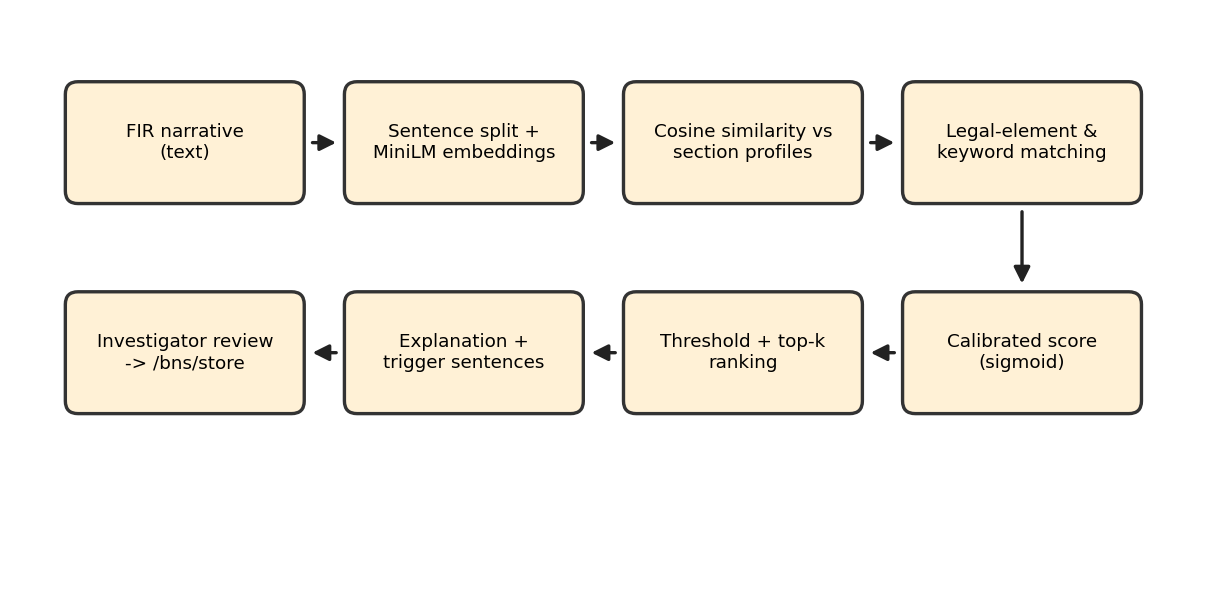
\includegraphics[width=15.0cm]{fig_bns_pipeline.png}
\caption{BNS decision-support pipeline}
\end{figure}

The gateway endpoint \code{POST /\allowbreak{}bns/\allowbreak{}predict} requires the \code{run\_\allowbreak{}ai\_\allowbreak{}analysis} permission, forwards the FIR text to the service and normalises the response; \code{POST /\allowbreak{}bns/\allowbreak{}store} saves the sections the investigator accepts in \code{bns\_\allowbreak{}predictions} after a case-access check, preserving earlier predictions, and both actions are audited. The repository also contains the research components of the RAG-HGAT classifier (a hierarchical graph attention model, a FAISS index of section embeddings, a rule-based post-processing layer and training data and results), which were used in the model study reported in Chapter 8.

\section{Audio Forensics Module}
The audio service (\code{audio-backend/\allowbreak{}app.py}) analyses an uploaded recording and returns a JSON report. The gateway route \code{POST /\allowbreak{}ai/\allowbreak{}audio/\allowbreak{}analyze} enforces permission, validates that any supplied evidence belongs to the stated case, forwards the file, and audits the run (ad-hoc runs without a case are labelled as such).

\begin{figure}[htbp]
\centering
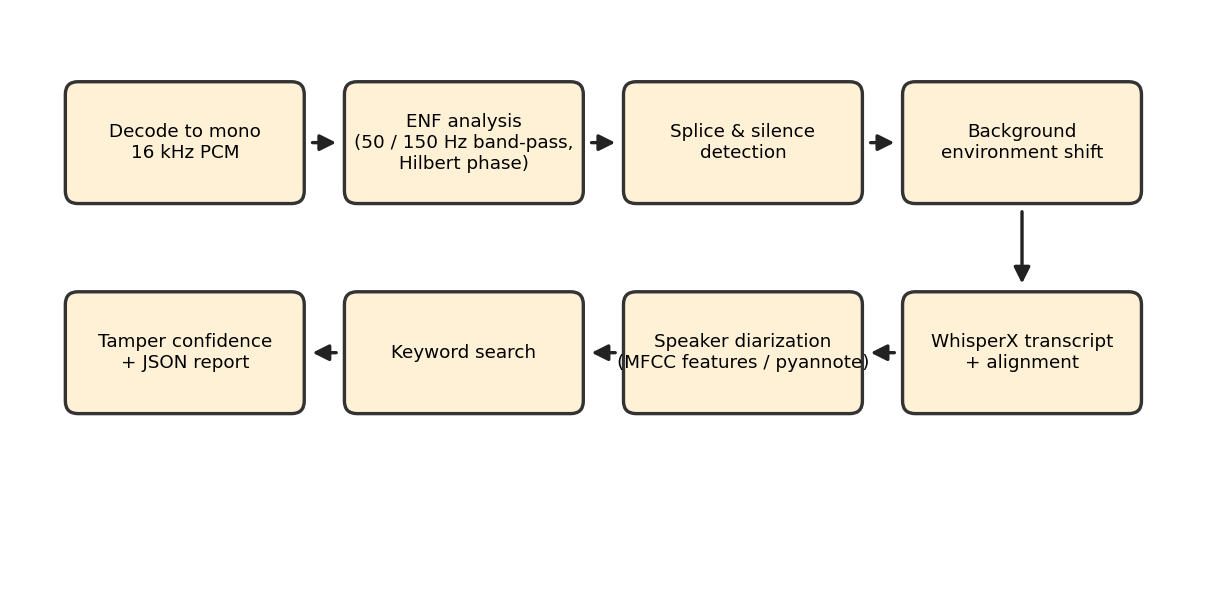
\includegraphics[width=15.0cm]{fig_audio_pipeline.png}
\caption{Audio forensics pipeline}
\end{figure}

\begin{itemize}
  \item \textbf{Decoding:} the container is decoded and converted to mono PCM at 16 kHz using native decoders or FFmpeg; metadata such as format, duration, sample rate, channels and bit depth are reported.
  \item \textbf{ENF analysis:} the signal is band-pass filtered around 50 Hz and its 150 Hz harmonic with a fourth-order Butterworth filter, the stronger band is selected, and the instantaneous frequency is obtained from the Hilbert-transform phase. A weak hum (energy ratio below 0.012) is reported as inconclusive rather than as evidence of tampering; otherwise a frequency step of 0.22 Hz or more between consecutive 0.2-second estimates is recorded as a discontinuity.
  \item \textbf{Splicing, silence and environment:} waveform step discontinuities, abrupt drops of the noise floor to digital zero, and shifts in background recording characteristics are detected from frame-level energy and spectral features.
  \item \textbf{Speech:} WhisperX produces a transcript with aligned word timestamps. Speakers are assigned using pyannote diarization when a Hugging Face token is configured, otherwise using clustering of acoustic features (20 MFCCs with deltas, spectral contrast, chroma, pitch, spectral centroid, roll-off and zero-crossing rate).
  \item \textbf{Keywords and verdict:} transcripts are searched for investigation-related keywords. A tampering confidence engine adds weighted indicators (ENF discontinuity, splicing cut, silence insertion, environment shift, speaker-profile shift) and reports an overall authenticity status in which a tampering verdict requires agreement between independent strong indicators.
  \item \textbf{Output:} the front end presents metadata, the ENF graph with highlighted discontinuities, speaker-attributed transcript segments, keywords and conclusions, and builds a printable forensic report.
\end{itemize}

\section{Photogrammetry Module}
The photogrammetry service turns a video evidence file into a 3D model. The gateway route \code{POST /\allowbreak{}photogrammetry/\allowbreak{}trigger/\allowbreak{}\{case\_\allowbreak{}id\}} verifies permission and case access, checks that the evidence belongs to the case and is a video, and calls the service with the evidence location. The service creates a job record in \code{photogrammetry\_\allowbreak{}models}, runs the pipeline in a background task and updates \code{current\_\allowbreak{}step} so that the interface can show live progress. Jobs left unfinished by a restart are marked Failed at start-up.

\begin{figure}[htbp]
\centering
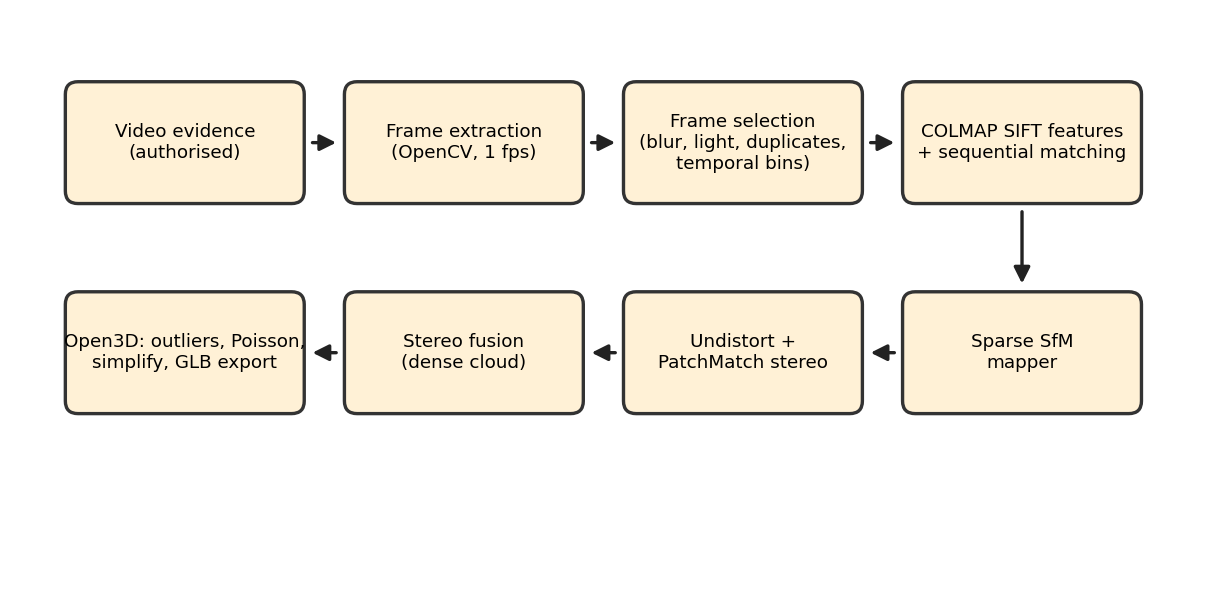
\includegraphics[width=15.0cm]{fig_photo_pipeline.png}
\caption{Photogrammetry processing pipeline}
\end{figure}

\begin{itemize}
  \item \textbf{Frame extraction:} OpenCV samples frames at a target rate (default one frame per second) from an optional time interval.
  \item \textbf{Frame selection:} frames are rejected if blurred (Laplacian variance below a threshold), too dark (mean HSV value), or near-duplicates of the previous accepted frame (normalised cross-correlation of down-scaled images). The remaining frames are divided into temporal bins, and the best-quality frame of each bin is kept so that the camera path remains continuous. Production and test modes use different thresholds.
  \item \textbf{COLMAP:} SIFT feature extraction (GPU), sequential matching, incremental mapping (SfM), image undistortion, PatchMatch stereo and stereo fusion produce a dense point cloud. Each stage has checkpoints so completed stages are skipped on resume, and a minimum camera-registration rate is enforced before dense reconstruction.
  \item \textbf{Open3D:} statistical outlier removal, normal estimation and orientation, Poisson surface reconstruction, cropping to the point-cloud bounds, removal of small disconnected components, quadric decimation (above 350,000 triangles), Taubin smoothing and colour transfer from the nearest points. Outputs are \code{model.ply}, \code{mesh.ply} and \code{model.glb}; the GLB header is validated.
  \item \textbf{Evaluation:} an evaluator computes registration rate, reprojection error, point counts and timing for each job, and a comparison summary across jobs is available through the API.
  \item \textbf{Delivery:} models are served through \code{GET /\allowbreak{}photogrammetry/\allowbreak{}model/\allowbreak{}\{job\_\allowbreak{}id\}/\allowbreak{}\{fmt\}} and displayed in the browser with Three.js.
\end{itemize}

\section{Investigation Aids}
\begin{itemize}
  \item \textbf{POLE graph:} \code{GET /\allowbreak{}cases/\allowbreak{}\{id\}/\allowbreak{}graph} builds nodes for the case, the FIR event, the incident location, each victim and suspect, and each evidence item, with labelled edges; the front end draws them with React Flow.
  \item \textbf{Notes:} personal notes are stored in a Supabase table, and the notes page provides a freehand canvas based on Excalidraw.
  \item \textbf{Dashboards:} \code{GET /\allowbreak{}cases/\allowbreak{}stats} supplies dashboard counts; \code{GET /\allowbreak{}blockchain/\allowbreak{}dashboard} and \code{/\allowbreak{}blockchain/\allowbreak{}ledger} supply network health, recent blocks, transactions and custody events, and \code{POST /\allowbreak{}blockchain/\allowbreak{}integrity-scan} (administrator) re-checks evidence and records failed checks.
  \item \textbf{User administration:} administrators create users in Supabase Auth with a temporary password that must be changed at first login, update roles and the case-creation right, activate or deactivate accounts and reset access.
\end{itemize}

\chapter{Algorithms and Technical Methods}
This chapter explains the main algorithms used by Secure Audit, why they were chosen and where they appear in the system.

\section{SHA-256 Hashing and Tamper Detection}
SHA-256 (FIPS 180-4) maps a file of any length to a 256-bit digest, written as 64 hexadecimal characters. It is deterministic, and a change to any bit of the input changes about half of the output bits (the avalanche effect), while finding a different file with the same digest is computationally infeasible. These properties make the digest a compact fingerprint of an exhibit.

\begin{equation*}
H = \mathrm{SHA\text{-}256}(F)
\end{equation*}

At upload, \code{H} is computed from the received bytes, compared with the digest produced by the storage provider, saved in \code{evidence.file\_\allowbreak{}hash} and registered on the blockchain. At verification, \code{H'} is recomputed from the stored object. The three values form the basis of the decision in Section 4.9:

\begin{equation*}
\text{Verified} \iff H' = H_{\mathrm{chain}}\ \ (\text{and } H_{\mathrm{db}} = H_{\mathrm{chain}};\ \text{otherwise DATABASE\_MISMATCH})
\end{equation*}

Checking the database copy as well as the file protects against an attacker who rewrites the stored hash but leaves the file unchanged; a check against the database alone would miss this case. In the evaluation, flipping one bit of a 31,965-byte image changed on average 127.85 of 256 digest bits over 1,000 trials, consistent with the ideal value of 128.

\section{Blockchain Anchoring and Event Synchronisation}
Only the digest and a few identifiers are written on-chain, so the cost per item is independent of file size and the evidence itself stays private. The contract's mapping from evidence ID to record, combined with write-once registration and append-only custody history, makes the registered value difficult to alter without detection. The gateway's listener repeats the following cycle: read events from the last processed block to the latest block, find the matching evidence by transaction hash or identifier, insert a custody record and a log row if they do not already exist, commit, and advance the cursor. Failures roll back the batch and are retried at the next poll.

\section{Hybrid OCR with Script-Aware Recognition}
PaddleOCR and Tesseract fail in complementary ways: Tesseract is stronger on some scripts (Kannada, and Malayalam where PaddleOCR has no model) but weaker on skewed or low-resolution pages, while PaddleOCR is a stronger general detector and layout source. The hybrid method therefore uses PaddleOCR for detection, orientation and layout, and re-reads individual line crops with the recogniser best suited to each script, accepting an alternative reading only if its confidence and own-script character ratio are better. Dropped digits in Tesseract output are restored from the PaddleOCR reading. Script detection counts characters per Unicode script block to label each line and page. Deskewing estimates the page angle by maximising the sharpness of a projection profile over candidate angles.

\section{BNS Retrieval and Scoring}
Let \code{d} be the normalised embedding of the whole narrative, \code{s\_\allowbreak{}i} the embeddings of its sentences and \code{p\_\allowbreak{}j} the normalised embedding of the profile of section \code{j}. Cosine similarity reduces to a dot product for unit vectors. For each section the service computes:

\begin{equation*}
d_{\mathrm{sim}} = \mathbf{d}\cdot \mathbf{p}_j, \qquad \max_s = \max_i\, (\mathbf{s}_i \cdot \mathbf{p}_j)
\end{equation*}

\begin{equation*}
\mathrm{raw} = 0.40\,\max_s + 0.25\,d_{\mathrm{sim}} + 0.35\,\mathrm{element\_score} \;(+\ \text{bonus for matched keywords or elements})
\end{equation*}

\begin{equation*}
\mathrm{confidence} = \frac{1}{1 + e^{-7(\mathrm{raw} - 0.40)}}, \quad \text{clipped to } [0.01,\,0.99]
\end{equation*}

\code{element\_\allowbreak{}score} measures how many of the statute's legal elements and keywords are present in the narrative, and a section with no matching element or keyword is skipped to avoid purely semantic false positives. The sigmoid maps raw scores to calibrated confidence values, sections at or above the threshold are ranked, and the best two sentences by similarity are shown as trigger sentences so that the investigator can see why a section was proposed. A separate post-processing module in the repository uses victim age, weapon, injury and offence-cluster rules with cluster thresholds to refine candidate lists.

\section{Object Detection with YOLOv8}
YOLOv8 is a single-stage detector that predicts class probabilities and bounding boxes in one forward pass, followed by non-maximum suppression (NMS). Predictions below the confidence threshold are discarded, and NMS removes overlapping boxes of the same class using the intersection over union:

\begin{equation*}
\mathrm{IoU}(B_1,B_2) = \frac{\mathrm{Area}(B_1 \cap B_2)}{\mathrm{Area}(B_1 \cup B_2)}
\end{equation*}

The gateway converts boxes to percentages of image width and height, so overlays remain correct at any display size.

\section{ENF Analysis and Audio Tampering Indicators}
Mains-powered recording equipment picks up a hum at the grid frequency (50 Hz in India) whose small frequency variations form a time-varying signature. After band-pass filtering at 50 Hz and 150 Hz, the analytic signal is formed with the Hilbert transform and the instantaneous frequency is the derivative of the unwrapped phase:

\begin{equation*}
f(t) = \frac{1}{2\pi}\,\frac{d\varphi(t)}{dt}, \qquad \varphi(t) = \mathrm{unwrap}\!\left(\arg\big(x(t) + j\,\mathcal{H}\{x(t)\}\big)\right)
\end{equation*}

The estimates are medianed over 0.2-second steps; a jump of at least 0.22 Hz between neighbours marks a candidate edit. Because ENF is fragile, other indicators (splice steps, digital silence, background changes, speaker-profile shifts) are weighted and combined, and a tampering verdict requires at least two strong indicators.

\section{Photogrammetry: SfM, MVS and Poisson Reconstruction}
Structure from Motion detects SIFT features in each selected frame, matches features between neighbouring frames, verifies matches geometrically and incrementally estimates camera poses and a sparse 3D point set by bundle adjustment, which minimises the reprojection error, i.e. the pixel distance between observed features and the projections of their estimated 3D points. Multi-view stereo (PatchMatch) estimates a depth map for each registered image and stereo fusion merges them into a dense coloured point cloud. Poisson surface reconstruction fits a smooth, watertight surface by solving for an indicator function whose gradient best matches the point normals; low-density regions and small isolated components are then removed. Frame selection with a Laplacian-variance sharpness test and temporal binning supplies sharp views with sufficient baseline.

\section{Storage-Key Validation and Stream Hashing}
Storage keys are canonicalised before use: backslashes are normalised, and keys that are empty, absolute, contain a drive letter or contain \code{.}, \code{..} or empty segments are rejected. Names are sanitised to a restricted character set and truncated, and identifiers are re-serialised from parsed UUIDs. Hashes are computed over streamed chunks so that large files do not need to be held twice in memory during verification.

\section{POLE Graph Generation}
The Person-Object-Location-Event model represents a case as a graph. Victims and suspects are Person nodes on opposite sides of the case node, evidence items are Object nodes, the incident location is a Location node and the FIR is an Event node. Positions are assigned deterministically so that the layout is stable between visits, and the status of each evidence item is displayed on its node.

\chapter{Testing and Validation}
\section{Testing Objectives}
\begin{itemize}
  \item Verify authentication, role-based access and case-ownership checks.
  \item Verify evidence hashing, duplicate handling, storage immutability and path-traversal protection.
  \item Verify blockchain registration, verification and custody behaviour, including tamper, missing-file and outage cases.
  \item Verify the behaviour of OCR rules, translation fallbacks and the analysis gateways under invalid input.
  \item Validate the accuracy and behaviour of the analysis modules on representative evidence.
\end{itemize}

\section{Testing Approach}
Testing combines unit tests of pure logic (integrity rules, OCR text handling, storage providers), contract tests of EvidenceRegistry against a local chain, API tests of the gateway using the FastAPI test client with mocked services, integration tests that exercise running services, and experimental evaluation of the analysis modules on prepared datasets. Tests are written with \code{unittest} or \code{pytest} conventions and live beside the services they test.

{\footnotesize
\setlength{\tabcolsep}{3pt}
\renewcommand{\arraystretch}{1.15}
\begin{longtable}{|>{\raggedright\arraybackslash}p{5.11cm}|>{\raggedright\arraybackslash}p{2.08cm}|>{\raggedright\arraybackslash}p{7.01cm}|}
\caption{Automated test suites in the repository}\\
\hline
\rowcolor{headfill}\textbf{Suite (location)} & \textbf{Test functions} & \textbf{Scope} \\ \hline
\endfirsthead
\hline
\rowcolor{headfill}\textbf{Suite (location)} & \textbf{Test functions} & \textbf{Scope} \\ \hline
\endhead
\hline \endfoot
test\_evidence\_integrity & 11 & Integrity checks and summaries, reason codes, hex normalisation \\ \hline
test\_deep\_integrity\_verification & 14 & Byte-level verification, metadata mismatch, missing and unreadable objects, fast-check API \\ \hline
test\_evidence\_registry\_contract & 8 & Registration, duplicates, input validation, registrar-only writes, verification events, custody actions, absence of delete \\ \hline
test\_blockchain\_api\_e2e & 1 & End-to-end evidence registration and verification through the API \\ \hline
test\_storage\_gateway & 9 & Put/get round trip, write-once refusal, traversal rejection, filename sanitisation, local path resolution \\ \hline
test\_cloud\_storage\_provider & 13 & S3-compatible provider with mocked client: permission errors, outages, missing objects, collisions \\ \hline
test\_storage\_migration\_e2e, test\_r2\_* & 7, 9, 10 & Migration dry-run and cloud connection tests (require configured storage) \\ \hline
test\_phase1\_security & 9 & Restrict foreign keys, audit buffering, blocked direct uploads path, role permissions \\ \hline
test\_audio\_security & 12 & 401/403/400/404/502 handling and case--evidence consistency in the audio gateway \\ \hline
test\_photogrammetry\_evidence\_status, test\_photogrammetry\_storage & 9, 12 & Reconstruction status routing, case isolation, model storage \\ \hline
test\_ocr\_text, test\_ocr\_engine\_rules & 25, 6 & Language detection, cleaning, layout rules, digit restoration, reading selection \\ \hline
test\_translation & 9 & Provider fallback, rate-limit handling, partial failure, long-line splitting \\ \hline
test\_best\_detection\_integration & 2 & Detection service health and inference on sample images \\ \hline
Audio, photogrammetry and BNS service tests & 7, 6, --- & Audio analysis, frame extraction/selection, COLMAP checkpointing; BNS validation scripts with benchmark output \\ \hline
\end{longtable}
}

\section{Integrity Test Scenarios}
The integrity tests cover the attack and failure scenarios listed in Table 13. In the end-to-end test campaign, all 17 automated checks across these scenarios produced the expected outcome.

{\footnotesize
\setlength{\tabcolsep}{3pt}
\renewcommand{\arraystretch}{1.15}
\begin{longtable}{|>{\raggedright\arraybackslash}p{6.63cm}|>{\raggedright\arraybackslash}p{5.21cm}|>{\raggedright\arraybackslash}p{2.37cm}|}
\caption{Integrity scenarios and expected outcomes}\\
\hline
\rowcolor{headfill}\textbf{Scenario} & \textbf{Expected outcome} & \textbf{HTTP status} \\ \hline
\endfirsthead
\hline
\rowcolor{headfill}\textbf{Scenario} & \textbf{Expected outcome} & \textbf{HTTP status} \\ \hline
\endhead
\hline \endfoot
Untouched file & Verified & 200 \\ \hline
File bytes modified or replaced & Tampered & 200 \\ \hline
Stored file path redirected to another file & Tampered & 200 \\ \hline
File deleted from storage & Missing & 404 \\ \hline
Database hash rewritten, file untouched & Verified with database-mismatch warning & 200 \\ \hline
Evidence never anchored on the chain & Unregistered & 409 \\ \hline
Client-supplied hash for a tampered item & Evidence status unchanged & 200 \\ \hline
Blockchain node unreachable & Structured error; evidence status unchanged & 503 \\ \hline
\end{longtable}
}

\section{Boundary and Error Testing}
\begin{itemize}
  \item Empty, oversized and unsupported files are rejected at upload or OCR; invalid UUIDs return HTTP 400 and unknown records return 404.
  \item Requests without a token return 401; requests without the required permission return 403; analysis of a case the user does not own returns 403.
  \item Evidence that does not belong to the stated case is rejected for audio, photogrammetry and detection requests.
  \item Unreachable analysis services return HTTP 502 and an unavailable blockchain returns HTTP 503, without corrupting database records.
  \item A video with too few usable frames, or a reconstruction with an insufficient camera-registration rate, fails with a descriptive error rather than producing an incomplete model.
  \item Missing files are distinguished from tampered files, and a verification attempt that fails because of an outage never changes the stored integrity state.
\end{itemize}

\section{Verification Run}
For this report, the suites that do not need external services were executed on the repository. \code{test\_\allowbreak{}evidence\_\allowbreak{}integrity} (11 tests) and \code{test\_\allowbreak{}ocr\_\allowbreak{}text} (25 tests) passed in full. In \code{test\_\allowbreak{}deep\_\allowbreak{}integrity\_\allowbreak{}verification}, 10 of 14 tests passed; the four tests of the fast-verification API need the gateway application to start with its Supabase configuration, which was not available in the environment used to prepare this report. Suites that require a running blockchain node, cloud storage credentials or analysis services were not re-executed for this document.

\chapter{Results and Discussion}
This chapter presents the results of the evaluation study carried out on the system and documented in the project's accompanying research paper (\code{paper/\allowbreak{}secure\_\allowbreak{}audit\_\allowbreak{}ieee.tex}) and benchmark files in the repository. OCR, BNS, audio and ledger experiments ran on an Intel Core i5-1335U laptop with 15.7 GB RAM and CPU-only inference; reconstruction ran on an NVIDIA GPU host; the ledger was a Ganache 7.9 node. The datasets are small and partly synthetic, as noted in the limitations below, and the figures should be read as indicators of behaviour rather than as field performance.

\section{Evidence Integrity and Blockchain}
All 17 automated integrity checks produced the expected outcome (Table 13). The database-only attack was detected because the verification compares the database hash with the chain hash. Registering an item costs 509,737 gas because every metadata string is stored on-chain, a verification call costs 142,733 gas in total (38,075 for \code{verifyEvidence} plus 104,658 for the custody entry), and the cost is independent of file size. The evaluation ledger held 77 custody events (24 registrations, 45 verifications, 8 transfers) for 24 evidence items, with no tampering among live case files (Figure 15).

\begin{figure}[htbp]
\centering
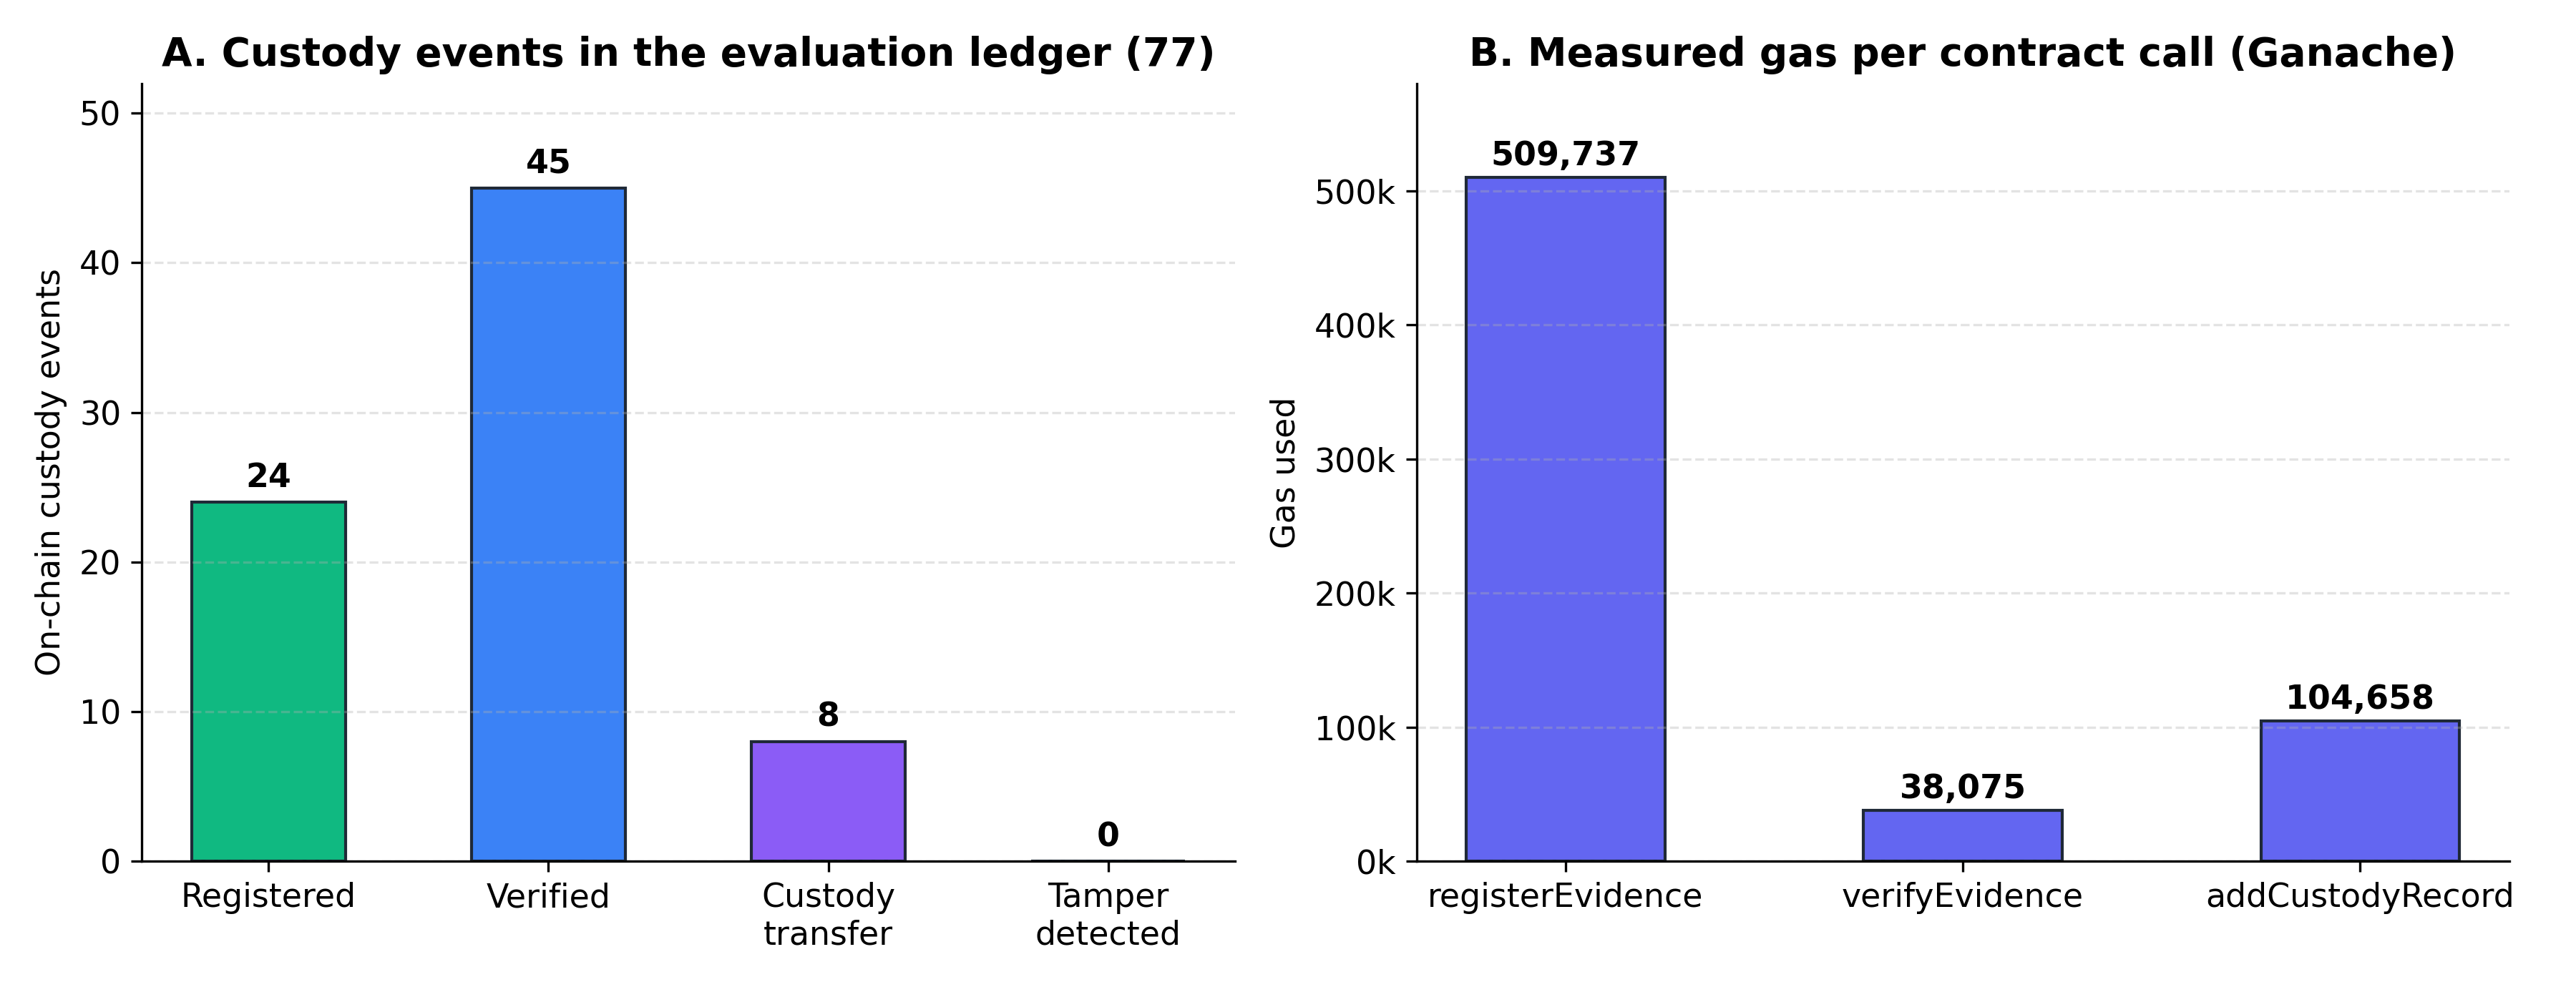
\includegraphics[width=15.0cm]{fig_blockchain_integrity.png}
\caption{Custody events in the evaluation ledger and measured gas per contract call}
\end{figure}

\section{Multilingual OCR}
OCR was evaluated on nine synthetic pages in six languages, including two mixed-script FIR layouts, under five conditions (clean, 0.4$\times$ downscaling, blur with noise, 3$^\circ$ skew and a simulated phone photograph). Hybrid OCR reduced the mean character error rate (CER) to 1.18\%, compared with 4.45\% for PaddleOCR and 4.17\% for Tesseract.

{\footnotesize
\setlength{\tabcolsep}{3pt}
\renewcommand{\arraystretch}{1.15}
\begin{longtable}{|>{\raggedright\arraybackslash}p{5.11cm}|>{\raggedright\arraybackslash}p{3.98cm}|>{\raggedright\arraybackslash}p{2.65cm}|>{\raggedright\arraybackslash}p{2.46cm}|}
\caption{Mean character error rate (\%) over five degradation conditions}\\
\hline
\rowcolor{headfill}\textbf{Document} & \textbf{PaddleOCR} & \textbf{Tesseract} & \textbf{Hybrid} \\ \hline
\endfirsthead
\hline
\rowcolor{headfill}\textbf{Document} & \textbf{PaddleOCR} & \textbf{Tesseract} & \textbf{Hybrid} \\ \hline
\endhead
\hline \endfoot
English & 0.00 & 0.00 & 0.00 \\ \hline
English (dense legal text) & 0.38 & 9.17 & 0.38 \\ \hline
Hindi & 1.50 & 0.00 & 1.50 \\ \hline
Kannada & 23.43 & 4.00 & 0.91 \\ \hline
Telugu & 4.89 & 4.24 & 4.78 \\ \hline
Tamil & 1.76 & 5.91 & 1.76 \\ \hline
Malayalam & --- & 10.16 & 0.65 \\ \hline
Mixed (EN+HI+KN) & 3.08 & 1.08 & 0.08 \\ \hline
Mixed (EN+TA+TE) & 0.59 & 3.00 & 0.59 \\ \hline
\textbf{Mean} & 4.45 (eight pages; no Malayalam model) & 4.17 & \textbf{1.18} \\ \hline
\end{longtable}
}

The engines fail in complementary ways, and giving each line to the recogniser best suited to its script brings Kannada from 23.43\% to 0.91\% and Malayalam to 0.65\%. Hindi remains on PaddleOCR because, on a real FIR, Tesseract truncated section numbers and times. Processing takes 2.5--3.3 s for a short page and 14.4--16.9 s for an 18-line trilingual page on CPU.

\section{BNS Decision Support}
The research RAG-HGAT classifier, trained on 10,000 template-generated cases (13 crime types, 57 sections, 70/15/15 split), reached a micro-F1 of 0.9871 and Hamming accuracy of 0.9988 on 1,500 held-out synthetic cases; because the data are template-generated, these scores mainly indicate fit to the generator. The deployed scorer was tested on 30 hand-written multi-offence FIRs with manually assigned sections (3.5 per case on average):

{\footnotesize
\setlength{\tabcolsep}{3pt}
\renewcommand{\arraystretch}{1.15}
\begin{longtable}{|>{\raggedright\arraybackslash}p{4.26cm}|>{\raggedright\arraybackslash}p{5.21cm}|>{\raggedright\arraybackslash}p{4.73cm}|}
\caption{BNS results}\\
\hline
\rowcolor{headfill}\textbf{Metric} & \textbf{RAG-HGAT (1,500 synthetic cases)} & \textbf{Deployed scorer (30 FIRs)} \\ \hline
\endfirsthead
\hline
\rowcolor{headfill}\textbf{Metric} & \textbf{RAG-HGAT (1,500 synthetic cases)} & \textbf{Deployed scorer (30 FIRs)} \\ \hline
\endhead
\hline \endfoot
Micro precision & 0.9835 & 0.369 \\ \hline
Micro recall & 0.9937 & 0.915 \\ \hline
Micro F1 & 0.9871 & 0.526 \\ \hline
Macro F1 & 0.9840 & 0.560 \\ \hline
Hamming accuracy & 0.9988 & --- \\ \hline
Crime-type accuracy & 0.9927 & --- \\ \hline
\end{longtable}
}

The deployed scorer recovered 97 of 106 gold sections (91.5\%) and missed no case entirely. Precision is low because about 8.8 sections are suggested per case; this is a deliberate trade-off, since a missed provision can weaken a charge sheet whereas a superfluous suggestion is dismissed quickly because it is shown with its trigger sentence. Classification takes about 85 ms per FIR.

\section{Audio Forensics}
The audio module was tested on 200 synthetic ten-second clips with two speaker pitches and five conditions. With a 220 Hz voice, all 40 authentic clips were judged authentic, every foreign insertion (2.0 s) and every digital-silence insertion was flagged. With a 140 Hz voice, speech energy near 150 Hz falls in the harmonic ENF band, so 39 of 40 authentic clips were marked as minor anomalies; because a tampering verdict needs two strong indicators, none was wrongly reported as tampered, while insertions (18/20) and silences (20/20) still escalated. Clean 1.3-second deletions at zero crossings went undetected with the 220 Hz voice, since the median filter smooths the short phase jump. A 60-second recording is analysed in about 4.2 s.

\section{3D Reconstruction}
Twenty-six reconstruction jobs were recorded (Table 16), mostly on a 65.5-second 4K walkthrough. Twenty produced complete meshes, three failed because of insufficient feature matches or textureless surfaces, and three stopped before dense reconstruction. Frame conditioning kept 960 of 1,892 extracted frames and COLMAP registered 732. The observation-weighted reprojection error over 1,996,707 observations was 0.8756 px (per-run median 0.837 px; Figure 16). After scaling with a known reference length, measurements of a footwear impression differed from ground truth by 0.33 cm on average (MAPE 2.97\%). A full 4K reconstruction takes about 31 minutes and is therefore run as a background job.

{\footnotesize
\setlength{\tabcolsep}{3pt}
\renewcommand{\arraystretch}{1.15}
\begin{longtable}{|>{\raggedright\arraybackslash}p{6.63cm}|>{\raggedright\arraybackslash}p{7.57cm}|}
\caption{Photogrammetry benchmark summary (26 jobs)}\\
\hline
\rowcolor{headfill}\textbf{Metric} & \textbf{Value} \\ \hline
\endfirsthead
\hline
\rowcolor{headfill}\textbf{Metric} & \textbf{Value} \\ \hline
\endhead
\hline \endfoot
Successful / failed / incomplete runs & 20 (76.9\%) / 3 (11.5\%) / 3 (11.5\%) \\ \hline
Keyframes selected / registered & 960 / 732 (weighted registration rate 76.25\%) \\ \hline
Observation-weighted reprojection error & 0.8756 px \\ \hline
Mean / median per-run reprojection error & 0.7942 px / 0.8369 px (range 0.49--1.32 px) \\ \hline
Sparse points triangulated & 362,233 \\ \hline
Fused dense points / after outlier removal & 15,861,223 / 12,800,584 \\ \hline
\end{longtable}
}

\begin{figure}[htbp]
\centering
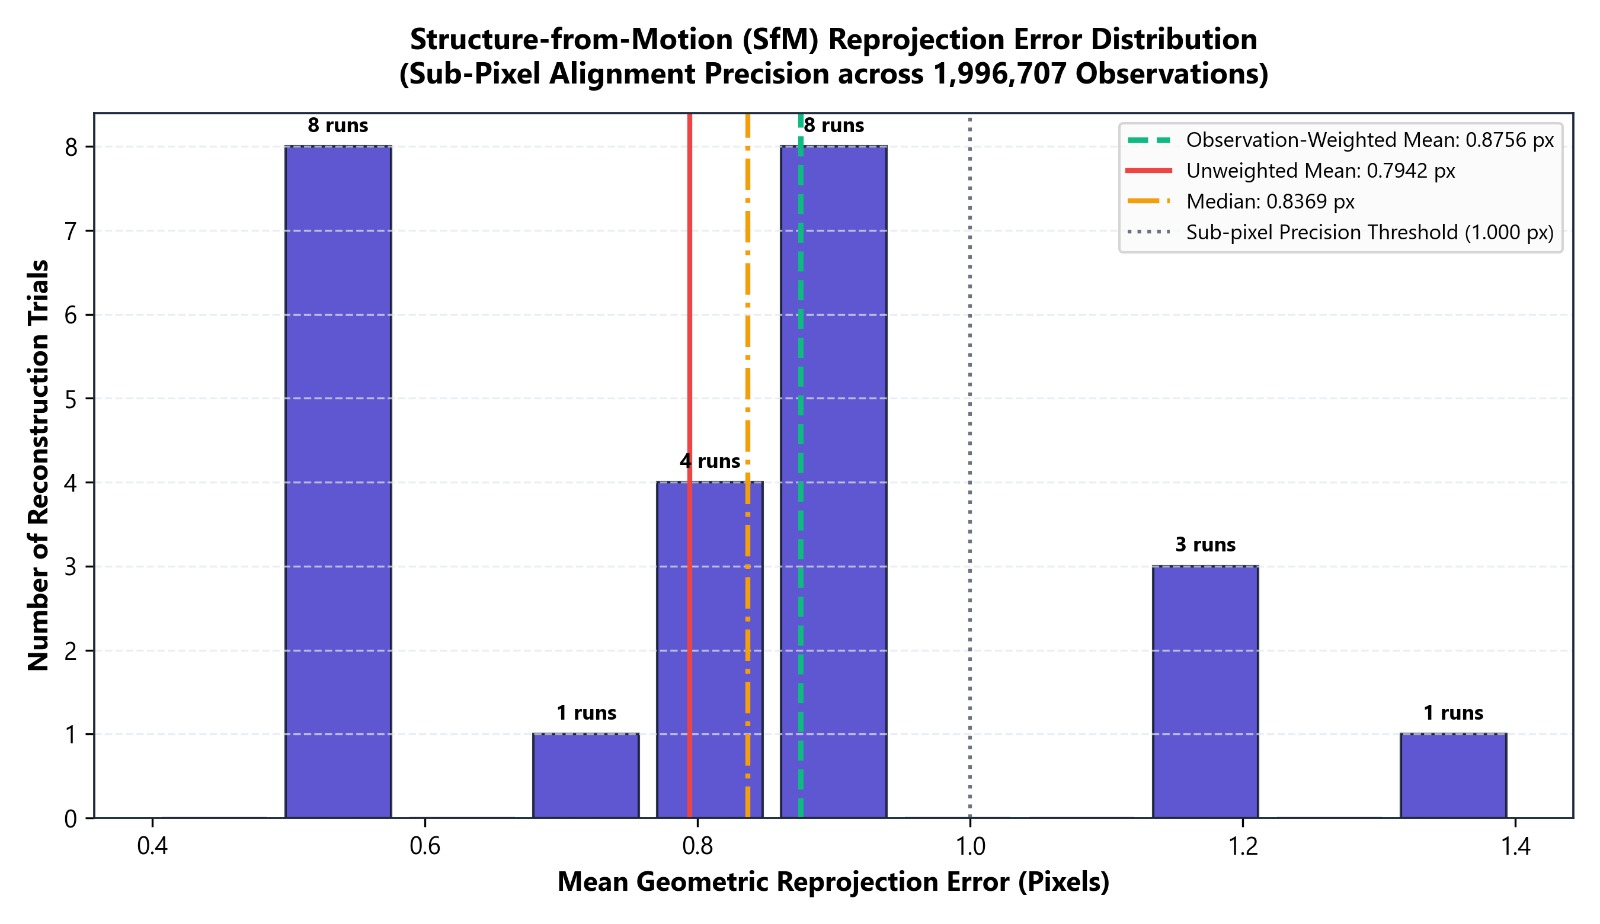
\includegraphics[width=13.5cm]{fig_reprojection_error.png}
\caption{Distribution of per-run mean reprojection error}
\end{figure}

\section{Discussion}
The results show that anchoring a digest before the database commit and comparing file, database and chain at verification detects every controlled tampering scenario, including database-only manipulation, at a fixed cost per item. The hybrid OCR design demonstrates the value of routing each line to the recogniser best suited to its script, and the BNS and audio modules are tuned toward the errors that matter most to an investigator: a minor anomaly is preferred to a false tampering accusation, and an extra suggestion to a missed charge. The 3D pipeline attains sub-pixel reprojection error on successful runs, with quality governed by viewpoint coverage, texture, lighting and blur.

The limitations of the evaluation should be noted. The BNS classifier and audio tests rely on template-generated narratives and synthetic edits, the OCR corpus is small with one typeface per script, the ledger was a single-node development network, and no field data from police records were used. Validation on de-identified real case material is the most important next step in assessing performance.

\chapter{Applications, Advantages and Limitations}
\section{Applications and Use Cases}
\begin{itemize}
  \item \textbf{Police stations and investigation units:} registering cases and FIRs, storing exhibits and keeping a defensible chain of custody.
  \item \textbf{Cyber and forensic laboratories:} verifying that analysed images, recordings and videos are identical to the collected exhibits.
  \item \textbf{Document examination:} extracting and translating text from multilingual, scanned or photographed FIRs and statements.
  \item \textbf{Scene documentation:} reconstructing a scene from a walkthrough video to review spatial relationships.
  \item \textbf{Audio evidence review:} checking recordings for signs of editing and producing speaker-attributed transcripts.
  \item \textbf{Legal triage:} suggesting candidate BNS sections with the supporting sentences for investigator review.
  \item \textbf{Audit and compliance review:} administrators reviewing the audit trail and running ledger integrity scans.
  \item \textbf{Teaching and research:} a reference implementation of a verifiable evidence workflow with integrated analysis.
\end{itemize}

\section{Advantages}
\begin{itemize}
  \item Independent integrity reference: digests are anchored on a blockchain before the database commit, so database manipulation does not go unnoticed.
  \item Distinct, explainable outcomes (Verified, Tampered, Missing, Unregistered) with reason codes, and outage results that never overwrite the evidence state.
  \item One authenticated workflow for evidence handling and analysis, with a common audit and custody trail.
  \item Provider-agnostic, write-once evidence storage with path-traversal protection and cloud support.
  \item Multilingual OCR for six languages with script-aware recognition and non-destructive translation.
  \item Explainable BNS suggestions that show trigger sentences, and audio verdicts that require corroborating indicators.
  \item Modular services that can be deployed, scaled and replaced independently.
\end{itemize}

\section{Limitations and Scope}
\begin{itemize}
  \item The shipped blockchain deployment is a single-node development network; production use calls for a permissioned or public network and key-management arrangements.
  \item Only evidence integrity is anchored on-chain; OCR text, translations and BNS suggestions are stored in the database and audited but not independently registered.
  \item The deployed BNS scorer covers 96 section entries and favours recall over precision; its output requires human review.
  \item ENF analysis is inconclusive for recordings without mains hum, and short clean deletions can escape detection.
  \item Reconstruction quality depends on coverage, texture and lighting, and dense reconstruction requires a CUDA GPU.
  \item The OCR and BNS evaluations use limited, partly synthetic data.
  \item The platform supports investigators; it does not replace forensic or judicial judgement.
\end{itemize}

\chapter{Conclusion}
Secure Audits: Digital Evidence and Investigation Support System demonstrates that evidence integrity and evidence analysis can be provided within a single, auditable workflow. Every uploaded file is fingerprinted with SHA-256, stored through a write-once storage gateway and registered in an Ethereum smart contract before its database record is committed. Verification compares the stored bytes with both the database and the blockchain and reports tampering, missing files, unregistered evidence and database manipulation as separate outcomes, while custody events and audit entries record how evidence is handled.

On top of this foundation, the platform offers hybrid multilingual OCR with optional translation, YOLOv8 object detection gated by an integrity check, explainable BNS decision support, forensic audio analysis based on ENF and corroborating indicators, and video-based 3D reconstruction with COLMAP and Open3D, together with a POLE graph, notes, dashboards and role-based user administration. The evaluation shows correct handling of all controlled integrity scenarios, a reduction of mean OCR character error rate from 4.45\% to 1.18\%, high recall of manually assigned BNS sections, and sub-pixel reprojection error in 3D reconstruction.

The system provides a structured basis for technology-assisted digital investigation. Its modular design allows the integrity gate to be applied to further services, the ledger to be moved to a permissioned network, and the analysis modules to be evaluated on larger, real-world forensic datasets.

\chapter*{References}
\addcontentsline{toc}{chapter}{References}
\begin{thebibliography}{99}
\setlength{\itemsep}{4pt}
\bibitem{r1} S. Bonomi, M. Casini, and C. Ciccotelli, ``B-CoC: A blockchain-based chain of custody for evidences management in digital forensics,'' in Int. Conf. Blockchain Economics, Security and Protocols (Tokenomics 2019), Schloss Dagstuhl -- Leibniz-Zentrum für Informatik, 2020, pp. 12:1--12:15, doi: 10.4230/OASIcs.Tokenomics.2019.12.
\bibitem{r2} M. Li, C. Lal, M. Conti, and D. Hu, ``LEChain: A blockchain-based lawful evidence management scheme for digital forensics,'' Future Generation Computer Systems, vol. 115, pp. 406--420, 2021.
\bibitem{r3} N. Sazaly et al., ``3D indoor crime scene reconstruction from micro UAV photogrammetry,'' Int. Arch. Photogramm. Remote Sens. Spatial Inf. Sci., vol. XLVIII-4/W6-2022, pp. 325--331, 2023.
\bibitem{r4} R. Balbudhe et al., ``Crime scene reconstruction: A scoping review,'' 2025.
\bibitem{r5} N. Mathias et al., ``Novel RAG-HGAT model for BNS section classification.''
\bibitem{r6} J. Kuok et al., ``CrimeKGQA: A crime investigation system based on knowledge graph RAG,'' 2024.
\bibitem{r7} A. Quyyum and N. Abdullah, ``Weapon detection in surveillance videos using deep neural networks,'' Journal of Intelligent \& Fuzzy Systems, vol. 44, no. 3, pp. 3891--3902, 2023.
\bibitem{r8} E. T. Ngharamike et al., ``ENF based digital multimedia forensics: Survey, application, challenges and future work,'' IEEE Access, vol. 11, 2023.
\bibitem{r9} S. Pedapudi and R. Vadlamani, ``Digital forensics approach for handling audio and video files,'' Int. Journal of Computer Applications, vol. 185, no. 12, 2023.
\bibitem{r10} M. A. Al Sayem et al., ``Implementing the Tesseract method for information extraction from images,'' Int. Journal of Advanced Computer Science and Applications, vol. 14, no. 5, 2023.
\bibitem{r11} P. Dhanushkumar et al., ``NLP and generative AI in law: A survey of AI-driven legal guidance for BNS,'' 2024.
\bibitem{r12} K. Werukanjana and P. Permpool, ``Integration of object detection in crime scene investigation,'' Applied Sciences, vol. 15, no. 3, Art. 1120, 2025.
\bibitem{r13} National Institute of Standards and Technology, ``Secure Hash Standard (SHS),'' FIPS PUB 180-4, 2015.
\bibitem{r14} G. Wood, ``Ethereum: A secure decentralised generalised transaction ledger,'' Ethereum Yellow Paper.
\bibitem{r15} G. Jocher, A. Chaurasia, and J. Qiu, ``Ultralytics YOLOv8,'' 2023. [Online]. Available: https://github.com/ultralytics/ultralytics
\bibitem{r16} R. Smith, ``An overview of the Tesseract OCR engine,'' in Proc. 9th Int. Conf. Document Analysis and Recognition (ICDAR), 2007, pp. 629--633.
\bibitem{r17} C. Cui et al., ``PaddleOCR 3.0 technical report,'' arXiv:2507.05595, 2025.
\bibitem{r18} N. Reimers and I. Gurevych, ``Sentence-BERT: Sentence embeddings using Siamese BERT-networks,'' in Proc. EMNLP-IJCNLP, 2019.
\bibitem{r19} I. Chalkidis et al., ``LEGAL-BERT: The muppets straight out of law school,'' in Findings of EMNLP, 2020.
\bibitem{r20} M. Bain, J. Huh, T. Han, and A. Zisserman, ``WhisperX: Time-accurate speech transcription of long-form audio,'' in Proc. Interspeech, 2023.
\bibitem{r21} J. L. Schönberger and J.-M. Frahm, ``Structure-from-motion revisited,'' in Proc. IEEE CVPR, 2016.
\bibitem{r22} J. L. Schönberger, E. Zheng, J.-M. Frahm, and M. Pollefeys, ``Pixelwise view selection for unstructured multi-view stereo,'' in Proc. ECCV, 2016.
\bibitem{r23} M. Kazhdan, M. Bolitho, and H. Hoppe, ``Poisson surface reconstruction,'' in Proc. Eurographics Symp. Geometry Processing, 2006.
\bibitem{r24} Q.-Y. Zhou, J. Park, and V. Koltun, ``Open3D: A modern library for 3D data processing,'' arXiv:1801.09847, 2018.
\bibitem{r25} S. Ramírez, ``FastAPI documentation.'' [Online]. Available: https://fastapi.tiangolo.com
\bibitem{r26} Government of India, ``The Bharatiya Nyaya Sanhita, 2023 (Act No. 45 of 2023).''
\end{thebibliography}

\end{document}
